\section{Perceptron}

%--------------------------------------------------------------------
\subsection{Perceptron linéaire}

\index{perceptron!lineaire@linéaire}

Le principe du perceptron linéaire est de prendre des valeurs en entrées, de faire un calcul simple et de renvoyer une valeur en sortie. Les calculs dépendent de paramètres propres à chaque perceptron.

\myfigure{1}{
	\tikzinput{fig_neurones_01}
}



Le calcul effectué par un perceptron se décompose en deux phases : un calcul par une fonction linéaire $f$, suivi d'une fonction d'activation $\phi$.

\myfigure{1}{
	\tikzinput{fig_neurones_02}
}


Détaillons chaque phase.
\begin{itemize}
	\item \textbf{Partie linéaire.} Le perceptron est d'abord muni de  \trouer{poids}\index{poids} $a_1,\ldots,a_n$
	qui déterminent une fonction linéaire 
	$$f(x_1,\ldots,x_n) = a_1 x_1 + a_2 x_2 + \cdots + a_n x_n.$$
	\item \textbf{Fonction d'activation.}\index{fonction d'activation} La valeur renvoyée par la fonction linéaire $f$ est ensuite composée par une fonction d'activation $\phi$.
	
	\item \textbf{Sortie.} La valeur de sortie est donc $\phi(a_1 x_1 + a_2 x_2 + \cdots + a_n x_n)$.
\end{itemize}

Dans ce chapitre, la fonction d'activation sera (presque) toujours la fonction marche de Heaviside :
$$\begin{cases}
	H(x) = 1 & \text{ si } x \ge 0, \\
	H(x) = 0  & \text{ si } x < 0. \\
\end{cases}$$

\myfigure{1}{
	\tikzinput{fig_neurones_04}
}



Voici ce que fait un perceptron linéaire de poids $a_1,\ldots,a_n$ et de fonction d'activation la fonction marche de Heaviside :

\myfigure{0.8}{
	\tikzinput{fig_neurones_03}
}


On peut donc définir ce qu'est un perceptron. Un   \trouer{perceptron linéaire} à $n$ variables et de fonction d'activation la fonction marche de Heaviside est la donnée de $n$ coefficients réels $a_1,\ldots,a_n$ auxquels est associée la fonction $F : \Rr \to \Rr$ définie par $F = H \circ f$, c'est-à-dire :
$$\begin{cases}
	F(x_1,\ldots,x_n) = 1 & \text{ si } a_1 x_1 + a_2 x_2 + \cdots + a_n x_n \ge 0, \\
	F(x_1,\ldots,x_n) = 0  & \text{ sinon.} \\
\end{cases}$$



\begin{exemple}{}{}
	
	Voici un perceptron à deux entrées. Il est défini par les poids $a=2$ et $b=3$.
	
	\myfigure{0.8}{
		\tikzinput{fig_neurones_05}
	}
	
	
	\begin{itemize}
		\item \textbf{Formule.}
		
		Notons $x$ et $y$ les deux réels en entrée.
		La fonction linéaire $f$ est donc 
		$$f(x,y) = 2x+3y.$$
		
		La valeur en sortie est donc :
		$$\begin{cases}
			F(x,y) = 1 & \text{ si } 2x+3y \ge 0 \\
			F(x,y) = 0  & \text{ sinon.} \\
		\end{cases}$$
		
		\myfigure{0.8}{
			\tikzinput{fig_neurones_06}
		}
		
		\item \textbf{\'Evaluation.} 
		Utilisons ce perceptron comme une fonction. Que renvoie le perceptron pour la valeur d'entrée $(x,y) = (4,-1)$ ?
		On calcule $f(x,y) = 2x+3y = 5$. Comme $f(x,y)\ge0$, alors la valeur de sortie est donc $F(x,y) = 1$.
		
		Recommençons avec $(x,y) = (-3,1)$. Cette fois $f(x,y) = -3 < 0$ donc $F(x,y) = 0$.
		
		L'entrée $(x,y) = (6,-4)$ est \og{}à la limite\fg{} car $f(x,y)=0$ ($0$ est l'abscisse critique pour la fonction marche de Heaviside).
		On a $F(x,y) = 1$.
		
		\item \textbf{Valeurs de la fonction.}
		
		La fonction $F$ prend seulement deux valeurs : $0$ ou $1$. La frontière correspond aux points $(x,y)$ tels que
		$f(x,y)=0$, c'est-à-dire à la droite $2x+3y=0$.  
		Pour les points au-dessus de la droite (ou sur la droite) la fonction $F$ prend la valeur $1$ ;
		pour les points en-dessous de la droite, la fonction $F$ vaut $0$.
		
		\myfigure{0.8}{
			\tikzinput{fig_neurones_07}
		}  
		
	\end{itemize}
\end{exemple}

\textbf{Notation.}

Nous représentons un perceptron par une forme plus condensée : 
sous la forme d'un   \trouer{neurone}, avec des poids sur les arêtes d'entrées. 
Nous précisons en indice la fonction d'activation utilisée  $\phi$.
Si le contexte est clair cette mention est omise.

\myfigure{0.7}{
	\tikzinput{fig_neurones_08}
}  

Voici le neurone à deux variables de l'exemple précédent.
\myfigure{0.7}{
	\tikzinput{fig_neurones_09}
}  

\begin{exemple}{}{}
	Voici deux catégories de points : des ronds bleus et des carrés rouges. Comment trouver un perceptron qui les sépare ?
	
	\myfigure{0.7}{
		\tikzinput{fig_neurones_10}
	} 
	
	Il s'agit donc de trouver les deux poids $a$ et $b$ d'un perceptron, dont la fonction associée
	$F$ vérifie $F(x,y)=1$ pour les coordonnées des carrés et $F(x,y)=0$ pour les ronds.
	
	\myfigure{0.7}{
		\tikzinput{fig_neurones_11}
	} 
	
	Trouvons une droite qui les sépare. Par exemple, la droite d'équation $4x-y=0$ sépare les ronds des carrés. On définit donc le neurone avec les poids $a=4$ et $b=-1$.
	Si $(x,y)$ sont les coordonnées d'un carré alors on a bien $F(x,y)=1$ et pour un rond $F(x,y)=0$.
	
	\begin{center}
		\begin{minipage}{0.35\textwidth}
			\myfigure{0.5}{
				\tikzinput{fig_neurones_12}
			}
		\end{minipage}
		\begin{minipage}{0.45\textwidth}
			\myfigure{0.6}{
				\tikzinput{fig_neurones_13}
			}
		\end{minipage}
	\end{center}
	
	
\end{exemple}

%--------------------------------------------------------------------
\subsection{Biais -- Perceptron affine}

Pour l'instant notre perceptron à deux entrées sépare le plan en deux parties selon une droite passant par l'origine.
Nous allons plus loin avec le  \trouer{perceptron affine}.\index{perceptron!affine@affine}

On modifie la définition du perceptron, sans changer le nombre d'entrées, mais en ajoutant un poids supplémentaire.
Dans le cas de $n$ entrées il y  a donc $n+1$  \trouer{poids} : 
\begin{itemize} 
	\item les  \trouer{coefficients} $a_1,\ldots,a_n \in \Rr$,
	\item et le  \trouer{biais}\index{biais} $a_0 \in \Rr$,
\end{itemize}
qui définissent la fonction affine :
$$f(x_1,\ldots,x_n) = a_1 x_1 + a_2 x_2 + \cdots + a_n x_n + a_0.$$
Comme auparavant, ce calcul est suivi de la fonction d'activation.


\myfigure{0.7}{
	\tikzinput{fig_neurones_14}
}

On représente le neurone avec une nouvelle arête, pondérée par le biais. L'arête  est terminée par un rond pour signifier que cela ne correspond pas à une entrée.

\myfigure{0.6}{
	\tikzinput{fig_neurones_15}
}


Dans le cas de deux entrées, les poids sont trois réels $a,b$ (les coefficients) et $c$ (le biais).
\myfigure{0.6}{
	\tikzinput{fig_neurones_16}
}

La fonction $f : \Rr^2 \to \Rr$ est la fonction affine $f(x,y) =ax+by+c$.
Si la fonction d'activation est la fonction marche de Heaviside, alors le perceptron affine définit une fonction $F : \Rr^2 \to \Rr$ par la formule :
$$\begin{cases}
	F(x,y) = 1 & \text{ si } ax+by+c \ge 0 \\
	F(x,y) = 0  & \text{ sinon.} \\
\end{cases}$$


Un perceptron affine à deux entrées sépare donc le plan en deux parties, la frontière étant la droite d'équation $ax+by+c=0$.
D'un côté de cette droite la fonction $F$ vaut $1$, de l'autre elle vaut $0$.

\myfigure{0.7}{
	\tikzinput{fig_neurones_17}
}

\begin{center}
	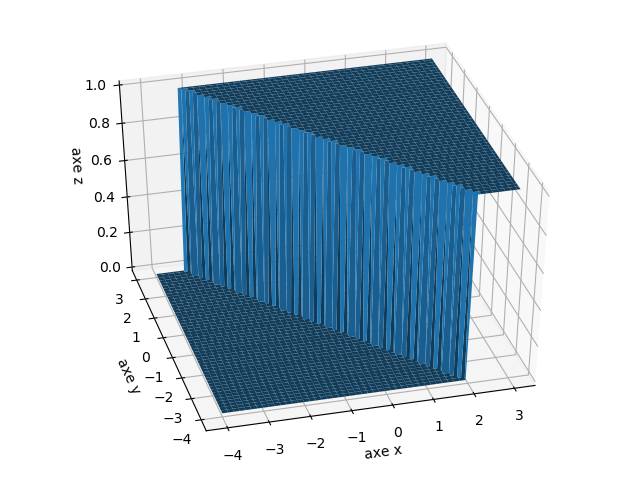
\includegraphics[scale=\myscale,scale=0.7]{figures/neurones-surface-4}
\end{center}



\begin{exemple}{}{}
	Trouver un perceptron qui distingue les carrés des ronds.
	\myfigure{0.7}{
		\tikzinput{fig_neurones_18}
	}
\end{exemple}


\bigskip

Il n'est pas toujours possible de répondre à une question seulement par \og{}oui\fg{} ou \og{}non\fg{}.
Pour y remédier, on peut changer de fonction d'activation en utilisant par exemple la fonction sigmoïde $\sigma$.
Dans ce cas, à chaque point du plan, on associe, non plus $0$ ou $1$, mais une valeur entre $0$ et $1$. 


Ce nombre peut correspondre à un degré de certitude. Par exemple avec une question \og{}Est-ce que cette photo est un chat ?\fg{}, si 
la sortie vaut $0.8$, cela signifie \og{}c'est bien un chat avec $80\%$ de certitude\fg{}. Si la sortie vaut $0.1$ alors ce n'est probablement pas un chat.

Voici un neurone à deux entrées muni de la fonction d'activation sigmoïde définie par $\sigma(x) = \frac{1}{1+e^{-x}}$.

\begin{center}
	\begin{minipage}{0.45\textwidth}
		\myfigure{0.5}{
			\tikzinput{fig_neurones_20}
		}
	\end{minipage}
	\begin{minipage}{0.45\textwidth}
		\myfigure{0.6}{
			\tikzinput{fig_neurones_19}
		}
	\end{minipage}
\end{center}

\begin{center}
	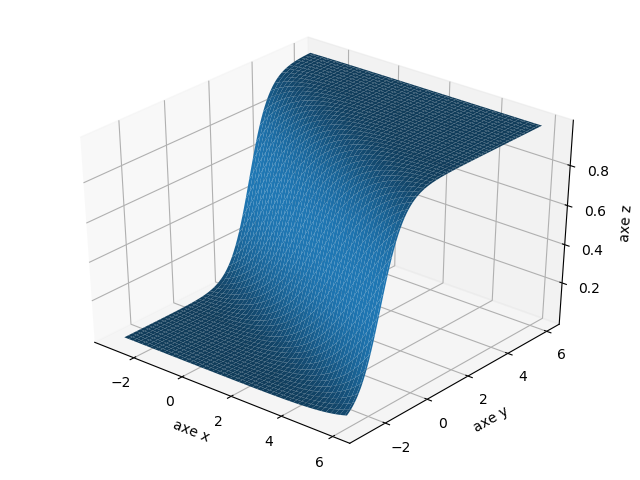
\includegraphics[scale=\myscale,scale=0.75]{figures/neurones-surface-3}
\end{center}


\begin{exemple}{}{}
	Voici les données (fictives) de la répartition des hommes et des femmes selon leur taille et leur poids.
	
	\myfigure{0.7}{
		\tikzinput{fig_neurones_21}
	}  
	
	
	Problème : la taille et le poids d'une personne étant donnés, trouver un perceptron qui réponde à la question \og{}Cette personne est-elle un homme ou une femme ?\fg{}.
	
	Au vu de la superposition des zones, il n'est pas possible de répondre avec certitude.  On construit donc un perceptron selon les idées suivantes :
	\begin{itemize}
		\item on trace une droite qui sépare au mieux les hommes des femmes, par exemple ici la droite qui passe par les points $A(1.40,42)$ et $B(2.00,93)$ d'équation approchée $y=85x-77$ où $(x,y)=(t,p)$ représente la taille et le poids ;
		
		\item on choisit la fonction d'activation sigmoïde.
	\end{itemize}
	Ce qui nous permet de définir le perceptron suivant avec $a=85$, $b=-1$ et $c=-77$.
	
	\begin{center}
		\begin{minipage}{0.35\textwidth}
			\myfigure{0.4}{
				\tikzinput{fig_neurones_22}
			}
		\end{minipage}
		\begin{minipage}{0.45\textwidth}
			\myfigure{0.7}{
				\tikzinput{fig_neurones_23}
			}
		\end{minipage}
	\end{center}
	
	Maintenant pour un couple donné $(t,p)$, le perceptron associe une valeur $F(t,p) \in [0,1]$.
	Si $F(t,p)$ est proche de $0$ alors la personne est probablement un homme, si $F(t,p)$ est proche de $1$ c'est probablement une femme.
	
	
	Exemple : une personne mesurant $1.77$\,m et pesant $75$\,kg est-elle plutôt un homme ou une femme ? On calcule $f(1.77,75)=-1.55$ où $f(x,y)=ax+by+c$.
	Puis on calcule $F(1.77,75) = \sigma(-1.55) \simeq 0.17$. Selon notre modèle cette personne est probablement un homme (car la valeur de $F$ est proche de $0$).
	
	Autre exemple : $(t,p)=(1.67,64)$. On calcule $F(1.67,64) \simeq 0.72$.
	Une personne mesurant $1.67$m et pesant $64$kg est probablement une femme (car la valeur de $F$ est plus proche de $1$ que de $0$).
	
	Malgré les données fictives, cet exemple met en évidence le problème de la superposition et de l'utilité d'avoir une sortie plus riche que  \og{}oui\fg{} ou \og{}non\fg{}. On peut aussi discuter de la pertinence de la frontière, car la séparation par une droite ne semble pas la mieux adaptée.  En fait, le poids varie en fonction du carré de la taille (les zones ont une forme de parabole). 
\end{exemple}




Plus généralement un  \trouer{perceptron affine} à $n$ entrées est la donnée de $n+1$ poids $a_0,a_1,\ldots,a_n \in \Rr$
et d'une fonction d'activation $\phi$ qui définissent une fonction $F : \Rr^n \to \Rr$
par la formule :
$$F(x_1,\ldots,x_n) = \phi(a_1 x_1 + \cdots + a_n x_n + a_0).$$

\begin{exemple}{}{}
	Dans le système de couleurs RGB (\emph{red, green, blue}), une couleur est déterminée par trois réels $r,g,b \in [0,1]$.
	Le \og{}vrai\fg{} rouge est codé par $(1,0,0)$, mais bien sûr des couleurs proches sont aussi des nuances de rouge.
	On représente toutes les couleurs par un \og{}cube de couleurs\fg{}, chaque point du cube représente le code $(r,g,b)$ d'une couleur.
	
	\myfigure{0.8}{
		\tikzinput{fig_neurones_24}
	}
	
	On décide (un peu arbitrairement) que toute couleur située dans la zone du coin $(1,0,0)$ de la figure ci-dessus est une nuance de rouge.
	
	Problème : trouver un perceptron qui répond à la question \og{}Cette couleur est-elle une nuance de rouge ?\fg{}.
	
	Solution. On considère que la zone est délimitée par le plan passant par les points $A(\frac12,0,0)$, $B(1,\frac12,0)$ et $C(1,0,\frac12)$ et les plans des faces du cube.
	Une équation de ce plan est $2x-2y-2z-1 = 0$ où en fait $(x,y,z)=(r,g,b)$.
	Le perceptron qui répond à la question est donc :
	
	\myfigure{0.7}{
		\tikzinput{fig_neurones_25}
	}
	
	La fonction $F$ associée, vérifie que $F(r,g,b) = 1$ pour les points de la zone des rouges et $F(r,g,b)=0$ sinon.
	
\end{exemple}



%%%%%%%%%%%%%%%%%%%%%%%%%%%%%%%%%%%%%%%%%%%%%%%%%%%%%%%%%%%%%%%%%%%%%
\section{Théorie du perceptron}

%--------------------------------------------------------------------
\subsection{OU, ET, OU exclusif}

\textbf{OU.}
Un  \trouer{booléen} est une variable qui peut prendre soit la valeur \og{}vrai\fg{}, soit la valeur \og{}faux\fg{}. 
Dans la pratique, on associe $1$ à \og{}vrai\fg{} et $0$ à \og{}faux\fg. \`A partir de deux booléens $x$ et $y$, on peut associer un nouveau booléen
\og{}$x$ OU $y$\fg{} qui est vrai lorsque $x$ est vrai ou $y$ est vrai.

Graphiquement, on représente toutes les configurations associées à \og{}$x$ OU $y$\fg{} par un diagramme. Un rond bleu en position $(x,y)$ signifie que \og{}$x$ OU $y$\fg{} est faux (le résultat vaut $0$), un carré rouge que \og{}$x$ OU $y$\fg{} est vrai (le résultat vaut $1$).

\myfigure{1}{
	\tikzinput{fig_neurones_26}
}


Peut-on réaliser l'opération \og{}$x$ OU $y$\fg{} par un perceptron ? 
Oui ! Cela revient à séparer les ronds bleus des carrés rouges.
C'est possible avec le perceptron de poids $a=1$, $b=1$, $c=-1$.
Par exemple, si $x=0$ et $y=1$ alors, on calcule $1\cdot0+1\cdot1-1 = 0 \ge0$. Composée avec la fonction marche de Heaviside, la fonction $F(x,y)$
définie par le perceptron renvoie dans ce cas $1$ (\og{}vrai\fg{}).
Si $x=0$ et $y=0$, alors $1\cdot0+1\cdot0-1 = -1 <0$ et $F(x,y)=0$ (\og{}faux\fg{}).

\begin{center}
	\begin{minipage}{0.35\textwidth}
		\myfigure{0.4}{
			\tikzinput{fig_neurones_27}
		}
	\end{minipage}
	\begin{minipage}{0.45\textwidth}
		\myfigure{0.7}{
			\tikzinput{fig_neurones_28}
		}
	\end{minipage}
\end{center}


\bigskip
\textbf{ET.}
On peut également réaliser l'opération \og{}$x$ ET $y$\fg{} (qui renvoie \og{}vrai\fg{} uniquement si $x$ et $y$ sont vrais) en choisissant les poids $a=1$, $b=1$, $c=-2$.

\begin{center}
	\begin{minipage}{0.35\textwidth}
		\myfigure{0.4}{
			\tikzinput{fig_neurones_29}
		}
	\end{minipage}
	\begin{minipage}{0.45\textwidth}
		\myfigure{0.7}{
			\tikzinput{fig_neurones_30}
		}
	\end{minipage}
\end{center}

%\begin{remarque*}
	D'un point de vue numérique, si on considère des valeurs réelles pour $x$ et $y$, notre perceptron \og{}ET\fg{} n'est pas numériquement très stable.
	Par exemple avec $x=0.9$ et $y=0.9$, on calcule $x+y-2=-0.2$ et la sortie est $0$, mais comme $x$ et $y$ sont proches de $1$, on aimerait que la sortie soit $1$.
	Il suffit de changer un peu les paramètres : prenons $a=1$, $b=1$ et $c=-1.5$, alors $x+y-1.5=0.3$ et cette fois la sortie est $1$.
%\end{remarque*}

\bigskip
\textbf{OU exclusif.}\index{ou exclusif}
Le ou exclusif, noté \og{}$x$ OUex $y$\fg{} est vrai lorsque $x$ ou $y$ est vrai, mais pas les deux en même temps. Le ou exclusif est-il réalisable par un perceptron ? Cette fois la réponse est non !

\myfigure{1}{
	\tikzinput{fig_neurones_31}
}


\begin{proposition}{}{}
	Il n'existe pas de perceptron (affine, à deux entrées et de fonction d'activation la fonction marche de Heaviside) qui réalise le \og{}ou exclusif\fg{}.
\end{proposition}

Nous sommes convaincus géométriquement qu'il n'existe pas de droite qui sépare les ronds bleus des carrés rouges. Nous allons le prouver par un petit calcul.

\begin{proof}
	Nous raisonnons par l'absurde en supposant qu'un tel perceptron existe. Nous cherchons une contradiction. 
	Soit $a_1=a,a_2=b,a_0=c$ les coefficients.
	
	\begin{center}
		\begin{minipage}{0.35\textwidth}
			\myfigure{0.4}{
				\tikzinput{fig_neurones_32}
			}
		\end{minipage}
		\begin{minipage}{0.45\textwidth}
			\myfigure{0.6}{
				\tikzinput{fig_neurones_33}
			}
		\end{minipage}
	\end{center}
	
	\begin{itemize}
		\item Pour $(x,y)=(1,0)$, on doit avoir $ax+by+c\ge0$ (car après avoir composé avec la fonction d'activation le résultat doit être $1$), 
		donc 
		\begin{equation}
			\label{eq:neur1}
			a+c \ge 0.
		\end{equation}
		\item De même pour $(x,y)=(0,1)$, on doit avoir $ax+by+c\ge0$, ce qui donne :
		\begin{equation}
			\label{eq:neur2}
			b+c \ge 0.
		\end{equation}
		\item Pour $(0,0)$ et $(1,1)$, on a $ax+by+c<0$, ce qui implique :
		\begin{equation}
			\label{eq:neur3}
			c<0,
		\end{equation}  
		\begin{equation}
			\label{eq:neur4}
			a+b+c<0.
		\end{equation}
	\end{itemize}
	
	Si on additionne les inégalités (\ref{eq:neur1}) et (\ref{eq:neur2}), on obtient $a+b+2c\ge0$. Par l'inégalité (\ref{eq:neur3}) on a $-c>0$. Donc en ajoutant $-c$ à l'inégalité $a+b+2c\ge0$, on obtient $a+b+c>0$. Ce qui contredit l'inégalité  (\ref{eq:neur4}).
	
	Conclusion : il ne peut exister trois réels $a,b,c$ pour définir un perceptron réalisant le \og{}ou exclusif\fg{}.
	
\end{proof}


%--------------------------------------------------------------------
\subsection{Séparation linéaire}

Nous formalisons un peu les idées de la section précédente.
Une  \trouer{droite} du plan $\Rr^2$ est l'ensemble des points $(x,y)$ vérifiant une équation du type $ax+by+c=0$. Un  \trouer{plan} de l'espace $\Rr^3$ est l'ensemble des points $(x,y,z)$ vérifiant une équation du type $ax+by+cz+d=0$.  Nous généralisons cette notion en dimension plus grande.
\begin{definition}{}{}
	Un  \trouer{hyperplan (affine)} de $\Rr^n$ est l'ensemble des points $(x_1,\ldots,x_n)$ qui vérifient une équation du type :
	$$a_1 x_1 + a_2 x_2 + \cdots + a_n x_n + a_0=0$$
	où $a_1,\ldots,a_n$ sont des réels (non tous nuls) et $a_0$ est aussi un réel.
\end{definition}


Le but d'un perceptron affine est de séparer deux ensembles. Par exemple deux ensembles $A$ et $B$ du plan seront séparés par une droite, deux ensembles de l'espace sont séparés par un plan.

\begin{definition}{}{}
	Deux ensembles $A$ et $B$ sont  \trouer{linéairement séparables} s'il existe un hyperplan qui sépare $A$ de $B$. Plus précisément, s'il existe des réels  $a_0,a_1,\ldots,a_n$ tels que $a_1 x_1 + a_2 x_2 + \cdots + a_n x_n + a_0 \ge 0$ pour tout $(x_1,\ldots,x_n) \in A$ et $a_1 x_1 + a_2 x_2 + \cdots + a_n x_n + a_0 < 0$ pour tout $(x_1,\ldots,x_n) \in B$.
\end{definition}

\myfigure{0.7}{
	\tikzinput{fig_neurones_34}
}

Nous résumons ce qui précède dans le résultat suivant.
\begin{proposition}{}{}
	Deux ensembles $A$ et $B$ de $\Rr^n$ sont linéairement séparables si, et seulement si, il existe un perceptron affine dont la fonction $F$ vaut $1$ sur $A$ et $0$ sur $B$.
\end{proposition}

La preuve est simple : la fonction $f$ définie par un perceptron (avant activation) est une fonction affine :
$$f(x_1,\ldots,x_n) = a_1 x_1 + a_2 x_2 + \cdots + a_n x_n + a_0.$$
Si $f(x_1,\ldots,x_n) \ge 0$, alors après activation $F(x_1,\ldots,x_n)=1$, sinon $F(x_1,\ldots,x_n)=0$.


\begin{exemple}{}{}
	Réaliser \og{}$x$ OU $y$ OU $z$\fg{} revient à séparer par un plan le rond bleu des carrés rouges du cube suivant. Trouver l'équation d'un de ces plans donne donc les poids du perceptron qui conviennent. 
	
	\begin{center}
		\begin{minipage}{0.60\textwidth}
			\myfigure{0.65}{
				\tikzinput{fig_neurones_35}
			}
		\end{minipage}
		\begin{minipage}{0.39\textwidth}
			\myfigure{0.6}{
				\tikzinput{fig_neurones_36}
			}
		\end{minipage}
	\end{center}
	
\end{exemple}

\begin{exemple}{}{}
	Trouver le perceptron qui réalise  \og{}$x$ ET $y$ ET $z$\fg{}.
	\myfigure{0.7}{
		\tikzinput{fig_neurones_37}
	}
	
\end{exemple}

% \todo{Exercice td : comptages des cubes réalisables ou pas preuve d'un qui n'est pas réalisable.}



%--------------------------------------------------------------------
\subsection{Vocabulaire}

Résumons le vocabulaire utilisé ci-dessus ainsi que les termes anglais correspondant :

\begin{itemize}
	\item le \textbf{perceptron linéaire} ou \textbf{neurone artificiel}, a un biais qui vaut $0$, à la différence du \textbf{perceptron affine} pour lequel le biais est un réel quelconque ;
	
	\item les \textbf{poids} (\emph{weights}) ou \textbf{paramètres} sont les \textbf{coefficients} $a_1,\ldots,a_n$ auxquels s'ajoute le \textbf{biais} (\emph{bias}) (dans ce livre le biais est l'un des poids, ce qui n'est pas toujours le cas dans la littérature) ;
	
	\item un perceptron est la donnée des poids et d'une fonction d'activation ;
	
	\item chaque perceptron définit une fonction $F$ qui est la composée d'une \textbf{fonction affine} $f$ et d'une \textbf{fonction d'activation} $\phi$ ; 
	la fonction d'activation la plus utilisée dans ce chapitre est la fonction marche de Heaviside (\emph{step function}) ; 
	
	\item on utilise un perceptron lors d'une \textbf{évaluation} : pour une \textbf{entrée} (\emph{input})
	$(x_1,\ldots,x_n) \in \Rr^n$, on calcule la sortie (\emph{output}) $F(x_1,\ldots,x_n) \in \Rr$ (qui vaut $0$ ou $1$ dans le cas de la fonction marche de Heaviside).  
\end{itemize}


\myfigure{0.8}{
	\tikzinput{fig_neurones_99}
}


%%%%%%%%%%%%%%%%%%%%%%%%%%%%%%%%%%%%%%%%%%%%%%%%%%%%%%%%%%%%%%%%%%%%%
\section{Réseau de neurones}

Un neurone permet de séparer l'espace en deux parties, la frontière étant linéaire (avec deux entrées c'est une droite, avec trois entrées c'est un plan\ldots). Un neurone est trop élémentaire pour résoudre nos problèmes, par exemple il ne peut réaliser le \og{}ou exclusif\fg{}. Comment faire mieux ? En connectant plusieurs neurones !

%--------------------------------------------------------------------
\subsection{Couches de neurones}

Un  \trouer{réseau de neurones} est la juxtaposition de plusieurs neurones, regroupés par  \trouer{couches}. 

\myfigure{1}{
	\tikzinput{fig_neurones_38}
}



\`A un réseau de neurones on associe une fonction.
Si à la dernière couche la fonction ne contient qu'un seul neurone (voir ci-dessus), cette fonction est  
$F : \Rr^n \to \Rr$, $y = F(x_1,\ldots,x_n)$ où $(x_1,\ldots,x_n)$ est l' \trouer{entrée} et $y$ est la  \trouer{sortie}.
Sinon (voir ci-dessous), la fonction est  
$F : \Rr^n \to \Rr^p$, $(y_1,\ldots,y_p) = F(x_1,\ldots,x_n)$ où $(x_1,\ldots,x_n) \in \Rr^n$ est l'entrée et $(y_1,\ldots,y_p)$ est la sortie.

\myfigure{1}{
	\tikzinput{fig_neurones_39}
}


\begin{exemple}{}{}
	Voici un réseau de neurones à deux couches : $2$ neurones (perceptrons linéaires) sur la première couche (ayant pour fonction d'activation la fonction ReLU), $1$ neurone (perceptron affine) sur la seconde couche  (de fonction d'activation $H$).
	
	\myfigure{1}{
		\tikzinput{fig_neurones_40}
	}
	
	
	
	\begin{itemize}
		\item Si $x=4$ et $y=7$ alors on calcule la sortie de chaque neurone de la première couche. Ces sorties sont les entrées du neurone de la seconde couche.
		Pour le premier neurone, on effectue le calcul $2\cdot4+(-1)\cdot7 = 1 \ge0$, le réel étant positif la fonction ReLU le garde inchangé : le premier neurone renvoie la valeur $s_1=1$. Le second neurone effectue le calcul $(-3)\cdot4+2\cdot7 = 2 \ge0$ et renvoie $s_2=2$.
		Le neurone de la couche de sortie reçoit en entrées $s_1$ et $s_2$ et effectue le calcul $4\cdot 1+5\cdot 2-1 = 13\ge0$. La fonction d'activation étant $H$, ce neurone renvoie $1$.  
		Ainsi $F(4,7)=1$.
		
		\myfigure{1}{
			\tikzinput{fig_neurones_41}
		}
		
		
		\item Si $(x,y)=(3,2)$ alors $s_1=4$, par contre $s_2=0$ car $(-3)\cdot3+2\cdot2 = -5 <0$ et la fonction ReLU renvoie $0$ (on dit que le neurone ne s'active pas). Les entrées du dernier neurone sont donc $s_1=4$ et $s_2=0$, ce neurone calcule $4\cdot 4 + 5\cdot0-1=15\ge0$ et, après la fonction d'activation, renvoie $1$. 
		Donc $F(3,2)=1$.
		
		\item Vérifier que pour $(x,y)=(\frac1{10},\frac1{10})$ le premier neurone s'active, le second ne s'active pas (il renvoie $0$) et le dernier neurone renvoie $0$. Ainsi $F(\frac1{10},\frac1{10})=0$.
	\end{itemize}
\end{exemple}


%\begin{remarque*}
%	\sauteligne
	\begin{itemize}
		\item Chaque neurone est défini par ses poids et une fonction d'activation. Pour une couche donnée, on choisit toujours la même fonction d'activation. En général on choisit la même fonction d'activation pour tout le réseau, sauf peut-être pour la couche de sortie.
		
		\item Un neurone prend plusieurs valeurs en entrée mais ne renvoie qu'une seule valeur en sortie ! Si ce neurone est connecté à plusieurs autres neurones, il envoie la même valeur à tous.
		
		\myfigure{0.5}{
			\tikzinput{fig_neurones_42}
		}
		
		\item On peut relier un neurone à tous les neurones de la couche suivante (voir ci-dessous figure de gauche). On dit que la seconde couche  est  \trouer{dense} ou  \trouer{complètement connectée}. Mais on peut aussi choisir de ne relier que certains neurones entre eux (voir ci-dessous figure de droite). S'il n'y a pas d'arêtes du neurone $A$ vers le neurone $B$, c'est que la sortie de $A$ n'intervient pas comme entrée de $B$ (cela revient à imposer un poids nul entre ces deux neurones).
		
		\myfigure{0.8}{
			\tikzinput{fig_neurones_43}\qquad\qquad
			\tikzinput{fig_neurones_44}  
		}  
		
		
		
	\end{itemize}
%\end{remarque*}  

\begin{exemple}{}{}
	Pour le réseau de neurones représenté ci-dessous, calculer les valeurs de sortie $(Y_1,Y_2)$ pour chacune des entrées $(x,y,z)$ suivantes :
	$$(0,0,0) \quad (1,0,0) \quad (1,-1,1) \quad (3,2,1)$$
	
	\myfigure{0.8}{
		\tikzinput{fig_neurones_45}
	} 
	
	
	
	Trouver un $(x,y,z)$ tel que $Y_1=1$ et $Y_2=7$ (commencer par déterminer les valeurs de sorties $s_1$ et $s_2$ de la première couche).
	
	%Trouver $(x,y,z)$ tel que $Y_2$ soit nul, mais pas $Y_1$.
	Existe-t-il $(x,y,z)$ tel que $Y_2$ soit nul, mais pas $Y_1$ ?
\end{exemple}

%--------------------------------------------------------------------
\subsection{Exemples}


\'Etudions quelques exemples plus en détails. Au lieu de calculer la sortie $F(x,y)$ pour des valeurs données, nous allons calculer $F(x,y)$ quelque soit $(x,y)$.

\vspace*{-1ex}

\begin{exemple}{}{}
	Voici un réseau de $3$ neurones : deux sur la première couche et un sur la seconde. La fonction d'activation est partout la fonction marche de Heaviside.
	Combien vaut la fonction associée $F$ selon l'entrée $(x,y)$ ?
	
	\myfigure{0.8}{
		\tikzinput{fig_neurones_46}
	} 
	
	
	On commence par calculer les sorties des neurones de la première couche.
	Pour le premier neurone la sortie $s_1$ dépend du signe de $-x+3y$.
	Si $-x+3y \ge 0$ alors $s_1(x,y)=1$, sinon $s_1(x,y)=0$. Donc pour les points $(x,y)$ situés au-dessus de la droite d'équation $-x+3y=0$, on a $s_1(x,y)=1$.
	De même pour le second neurone, on a $s_2(x,y)=1$ pour les points situés au dessus de la droite $2x+y=0$. Voir la figure ci-dessous.
	\myfigure{0.6}{
		\tikzinput{fig_neurones_47}  
	} 
	On reconnaît dans le neurone de sortie un neurone qui réalise le \og{}ET\fg{}. 
	C'est pourquoi l'ensemble des points pour lesquels $F$ vaut $1$ est l'intersection des deux demi-plans en lesquels $s_1$ et $s_2$ valent $1$. Ainsi $F(x,y)=1$ dans un secteur angulaire et $F(x,y)=0$ ailleurs. Voir la figure ci-dessous.
	
	\myfigure{0.6}{
		\tikzinput{fig_neurones_48}  
	} 
	
\end{exemple}

\medskip

\begin{exemple}{}{}
	On reprend la même architecture que l'exemple précédent, mais en changeant les poids du neurone de sortie qui réalise cette fois l'opération \og{}OU\fg{}.
	
	\myfigure{0.8}{
		\tikzinput{fig_neurones_49}
	} 
	
	L'ensemble des points pour lesquels $F$ vaut $1$ est maintenant l'union des deux demi-plans en lesquels $s_1$ et $s_2$ valent $1$.
	
	\myfigure{0.6}{
		\tikzinput{fig_neurones_50}  
	} 
\end{exemple}

\begin{exemple}{}{}
	Voici un réseau de neurones un peu plus compliqué (la fonction d'activation est $H$ partout). 
	\myfigure{0.8}{
		\tikzinput{fig_neurones_51}
	} 
	
	Chaque neurone de la première couche délimite un demi-plan. Ce sont les demi-plans $-x+2y\ge0$, $x+y-2\ge0$ et $-y+3\ge0$.
	
	Le neurone de sortie est un neurone qui réalise l'opération \og{}ET\fg{} : il s'active uniquement si les trois précédents neurones sont activés.
	Ainsi la sortie finale $F(x,y)$ vaut $1$ si et seulement si $(x,y)$ appartient simultanément aux trois demi-plans.
	
	\myfigure{0.8}{
		\tikzinput{fig_neurones_52}  
	}
	
\end{exemple}

\begin{exemple}{}{}
	En utilisant les idées de l'exemple précédent et pour le dessin ci-dessous, trouver un réseau de neurones dont la fonction $F$ vaut $1$ pour la zone colorée et $0$ ailleurs.
	
	\myfigure{0.5}{
		\tikzinput{fig_neurones_53}  
	}
	
	
\end{exemple}


\begin{exemple}{}{}
	On termine en comparant les fonctions produites par des réseaux ayant la même architecture, les mêmes poids mais de fonction d'activation $\phi$ différente : $H$, $\sigma$, $\tanh$ et ReLU.
	
	\myfigure{0.8}{
		\tikzinput{fig_neurones_51bis}  
	}
	
	Voici les graphiques 3D obtenus pour les fonctions d'activation $H$ (comme dans l'exemple vu auparavant), $\sigma$, $\tanh$ et ReLU. Les fonctions $F$ obtenues dépendent fortement du choix de la fonction d'activation.
	
	\begin{center}
		\begin{minipage}{0.4\textwidth}
			\center
			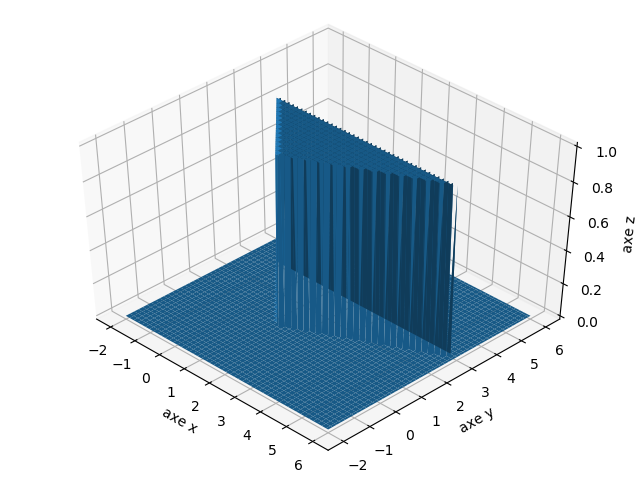
\includegraphics[scale=\myscale,scale=0.4]{figures/neurones-surface-2-heaviside}
			Activation $H$
		\end{minipage}\quad
		\begin{minipage}{0.4\textwidth}
			\center
			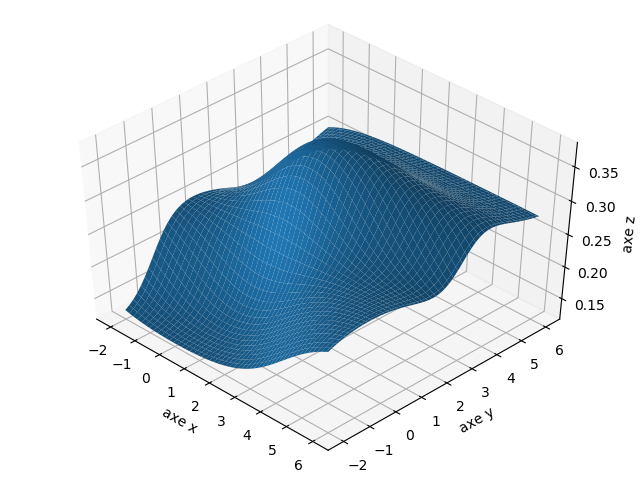
\includegraphics[scale=\myscale,scale=0.4]{figures/neurones-surface-2-sigma}
			Activation $\sigma$
		\end{minipage}
	\end{center}
	
	\begin{center}
		\begin{minipage}{0.4\textwidth}
			\center
			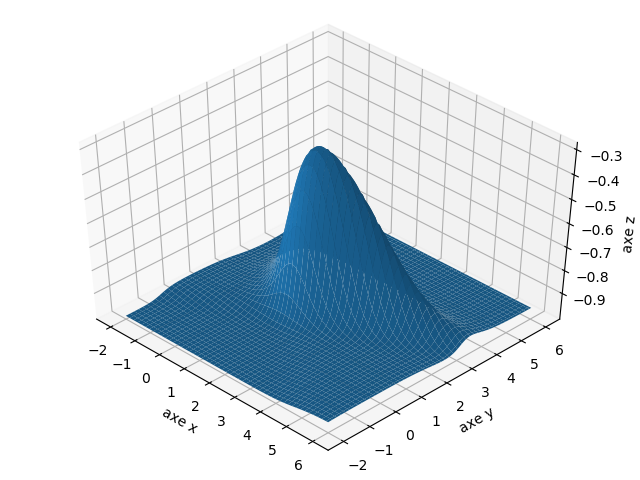
\includegraphics[scale=\myscale,scale=0.4]{figures/neurones-surface-2-tanh}
			Activation $\tanh$
		\end{minipage}\quad
		\begin{minipage}{0.4\textwidth}
			\center
			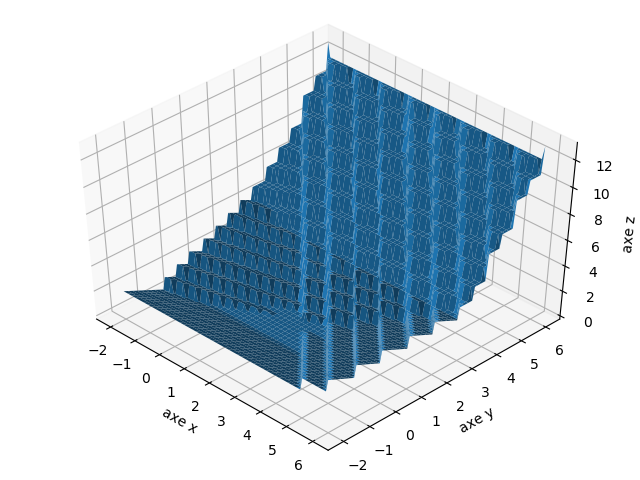
\includegraphics[scale=\myscale,scale=0.4]{figures/neurones-surface-2-relu}
			Activation ReLU
		\end{minipage}
	\end{center}
\end{exemple}


% \todo{Exercice td : rond bleu, carrés rouge avec trois droites}


% \todo{Exercice td : l'influence d'un poids sur la fonction générée par le réseau. à faire réseau 2+1, H, un coeff qui varie, i.e. une droite varie plusieurs dessins}

%%%%%%%%%%%%%%%%%%%%%%%%%%%%%%%%%%%%%%%%%%%%%%%%%%%%%%%%%%%%%%%%%%%%%
\section{Théorie des réseaux de neurones}

%--------------------------------------------------------------------
\subsection{OU exclusif}

Nous avons vu qu'un seul neurone ne permet pas de réaliser la fonction associée au \og{}OU exclusif\fg{}.
Avec plusieurs neurones c'est facile !
Voici un réseau de neurones qui sépare le plan en trois parties, le secteur central en lequel la fonction associée au réseau vaut $0$, alors que la fonction vaut $1$ partout ailleurs (y compris sur la frontière\couleurnb{ rouge}).
\myfigure{0.7}{
	\tikzinput{fig_neurones_54}
}

\myfigure{0.8}{
	\tikzinput{fig_neurones_55}
}



Ce réseau permet d'obtenir une valeur $F(x,y)=1$ en $(1,0)$ et $(0,1)$ et une valeur $F(x,y)=0$ en $(0,0)$ et $(1,1)$.

L'idée de ce réseau vient du fait que l'opération \og{}OU exclusif\fg{} est une combinaison de \og{}OU\fg{} et de \og{}ET\fg{} :
$$x \text{ OUex } y  = (x \text{ ET } \text{non} y) \text{ OU } ( \text{non} x \text{ ET } y).$$


\begin{center}
	\begin{minipage}{0.60\textwidth}
		\myfigure{0.9}{
			\tikzinput{fig_neurones_56}
		}
	\end{minipage}
	\begin{minipage}{0.39\textwidth}
		\myfigure{0.8}{
			\tikzinput{fig_neurones_31}
		}
	\end{minipage}
\end{center}

Le neurone du haut réalise \og{}$x \text{ ET } \text{non} y$\fg{}, le neurone du bas \og{}$\text{non} x \text{ ET } y$\fg{} et celui de sortie l'opération \og{}OU\fg{}.

%--------------------------------------------------------------------
\subsection{Ensemble réalisable}

Nous aimerions savoir quels ensembles peuvent être décrits par un réseau de neurones.
On rappelle qu'un ensemble $A \subset \Rr^2$ découpe le plan en trois parties disjointes : intérieur, frontière, extérieur :
$$\Int(A) \qquad \Fr(A) \qquad \Ext(A).$$

\myfigure{0.9}{
	\tikzinput{fig_neurones_57}
}

\begin{definition}{}{}
	Un ensemble $A$ est dit  \trouer{réalisable par un réseau de neurones} s'il existe un réseau de neurones $\mathcal{R}$ (d'unique fonction d'activation la fonction marche de Heaviside) tel que
	la fonction $F : \Rr^2 \to \Rr$ associée à $\mathcal{R}$ vérifie :
	$$F(x,y) = 1 \quad \text{ pour tout } (x,y) \in \Int(A)$$
	et
	$$F(x,y) = 0 \quad \text{ pour tout } (x,y) \in \Ext(A).$$
\end{definition}

\myfigure{0.9}{
	\tikzinput{fig_neurones_58}
}


Remarque : on n'exige rien sur la frontière $\Fr(A)$, $F$ peut y prendre la valeur $0$ ou la valeur $1$.


Voici les types d'ensembles que nous avons déjà réalisés :
\begin{itemize}
	\item les demi-plans,
	\item les \og{}quart de plans\fg{},
	\item les zones triangulaires,
	\item les triangles avec un sommet \og{}à l'infini\fg{}.
\end{itemize}

\myfigure{0.6}{
	\tikzinput{fig_neurones_59}
}


En augmentant le nombre de neurones, on peut réaliser les quadrilatères convexes et plus généralement n'importe quelle zone polygonale convexe.

\begin{proposition}{}{}
	Tout zone polygonale convexe à $n$ côtés est réalisable par un réseau de $n+1$ neurones.
\end{proposition}

\myfigure{0.6}{
	\tikzinput{fig_neurones_60}
}

\begin{proof}
	Un polygone convexe à $n$ côtés est l'intersection de $n$ demi-plans.
	Chaque demi-plan, bordé par une droite d'équation du type $ax+by+c=0$, correspond à un neurone de la première couche dont les coefficients sont $(a,b)$ et le biais est $c$ (ou alors $(-a,-b)$ et $-c$).
	Sur la seconde couche, on place un neurone qui réalise l'opération \og{}ET\fg{} sur les $n$ entrées : tous ses coefficients sont $1$ et le biais est $-n$.
\end{proof}

Continuons avec des opérations élémentaires sur les ensembles réalisables.
\begin{proposition}{}{}
	Si $A$ et $B$ sont deux ensembles du plan réalisables par des réseaux de neurones alors :
	$$A\cup B \qquad A\cap B \qquad A^\complement  \qquad A \setminus B$$
	sont aussi des ensembles réalisables. 
\end{proposition}


\myfigure{0.8}{
	\tikzinput{fig_neurones_61}
}


\begin{proof}
	~
	\begin{itemize}
		\item Si $A$ est réalisé par un réseau $\mathcal{R}_A$ et $B$ par un réseau  $\mathcal{R}_B$
		alors on crée un nouveau réseau $\mathcal{R}$ en superposant $\mathcal{R}_A$ et $\mathcal{R}_B$
		et en ajoutant un neurone \og{}OU\fg{} à partir des sorties de $\mathcal{R}_A$ et $\mathcal{R}_B$.
		Ainsi si $(x,y)$ est dans $A \cup B$, il est dans $A$ ou dans $B$, une des sorties  $\mathcal{R}_A$ ou $\mathcal{R}_B$ vaut alors $1$ et le neurone sortant de $\mathcal{R}$ s'active.
		
		\myfigure{0.8}{
			\tikzinput{fig_neurones_62}
		}
		
		
		\item Pour réaliser $A \cap B$, on remplace le neurone \og{}OU\fg{} par un neurone \og{}ET\fg{}.
		
		\myfigure{0.8}{
			\tikzinput{fig_neurones_63}
		}
		
		\item Pour réaliser le complément d'un ensemble $A$, on utilise l'opération \og{}non\fg{} : $0$ s'envoie sur $1$ et $1$ sur $0$. Ceci se fait par l'application 
		$s \mapsto H(1-2s)$. Il suffit juste de rajouter un neurone \og{}NON\fg{} à $\mathcal{R}_A$.
		
		\myfigure{0.8}{
			\tikzinput{fig_neurones_64}
		} 
		
		\item Comme $A \setminus B = A \cap \big((A\cap B)^\complement \big)$ alors 
		il est possible de réaliser $A \setminus B$ comme succession d'opérations élémentaires $\cap$, $\complement$ et $\cup$.
	\end{itemize}
	
	
\end{proof}

% [[Pb de la frontière? si $A$ réalisable alors $A\cup \Fr(A)$ *vraiment* réalisable et $A\setminus \Fr(A)$ aussi]]






\begin{proposition}{}{}
	Tout polygone (convexe ou non) est réalisable par un réseau de neurones.
\end{proposition}

\begin{proof}
	Un polygone peut être découpé en triangles. Chaque triangle est réalisable, donc l'union des triangles l'est aussi.
	
	\myfigure{0.8}{
		\tikzinput{fig_neurones_65}
	}
	
	
\end{proof}

%--------------------------------------------------------------------
\subsection{Approximation d'ensembles}



On rappelle qu'une  \trouer{courbe de Jordan} $C$ est une courbe fermée simple (c'est l'image d'un cercle par une application continue injective). Le théorème suivant est une sorte de théorème d'approximation universelle géométrique.
\myfigure{0.8}{
	\tikzinput{fig_neurones_66}
}

\begin{theoreme}{}{}
	Un ensemble $A$ délimité par une courbe de Jordan peut être approché d'aussi près que l'on veut par un ensemble $A'$ réalisable par un réseau de neurones.
\end{theoreme}

Il s'agit juste du fait qu'une courbe de Jordan peut être approchée par un polygone.
C'est un résultat théorique qui ne dit en rien comment choisir la structure du réseau ou les poids.

\myfigure{0.8}{
	\tikzinput{fig_neurones_67}
}

% [[Preuve voir Tverberg, A proof of the Jordan curve theorem, Bull London Math Soc, 1980]]



%%%%%%%%%%%%%%%%%%%%%%%%%%%%%%%%%%%%%%%%%%%%%%%%%%%%%%%%%%%%%%%%%%%%%
\section{Théorème d'approximation universelle}

Nous allons maintenant prouver qu'un réseau de neurones bien construit peut approcher n'importe quelle fonction. 

Dans cette section nous partirons d'une seule entrée $x \in \Rr$, avec une seule sortie $y = F(x) \in \Rr$. Les réseaux de neurones de cette section produisent donc des fonctions $F : \Rr \to \Rr$.

L'objectif est le suivant : on nous donne une fonction $f : [a,b] \to \Rr$ et nous devons trouver un réseau, tel que la fonction $F$ associée à ce réseau soit proche de $f$ :
$$F(x) \simeq f(x) \qquad \text{ pour tout } x \in [a,b].$$

Pour paramétrer le réseau nous allons bien sûr fixer des poids, mais avant cela choisissons les fonctions d'activation :
\begin{itemize}
	\item pour le neurone de sortie, on choisit la fonction identité $\phi(x)=x$,
	\item pour tous les autres neurones, on choisit la fonction marche de Heaviside.
\end{itemize}


%\begin{remarque*}
%	\sauteligne
	\begin{itemize}
		\item Si on choisissait aussi la fonction d'activation marche de Heaviside pour le neurone de sortie, alors $F$ ne pourrait prendre que deux valeurs, $0$ ou $1$, ce qui empêcherait de réaliser la plupart des fonctions.
		
		\item Par contre, si on choisissait la fonction identité pour tous les neurones alors on ne réaliserait que des fonctions affines $F(x)=ax+b$ (en effet la composition de plusieurs fonctions affines reste une fonction affine). 
		
	\end{itemize}
%\end{remarque*}

%--------------------------------------------------------------------
\subsection{Fonctions marches}
\label{ssec:marches}

Nous allons réaliser des fonctions de plus en plus compliquées à partir d'éléments très simples.


Commençons par étudier le comportement d'un seul neurone avec la fonction d'activation marche de Heaviside (on rajoutera le neurone de sortie plus tard).

Voici différents neurones et les fonctions qu'ils réalisent :
\begin{itemize}
	\item La fonction marche de Heaviside.
	
	\begin{center}
		\begin{minipage}{0.35\textwidth}
			\myfigure{0.9}{
				\tikzinput{fig_neurones_68}
			}
		\end{minipage}
		\begin{minipage}{0.59\textwidth}
			\myfigure{0.7}{
				\tikzinput{fig_neurones_69}
			}
		\end{minipage}
	\end{center}  
	
	
	\item La fonction marche décalée vers la gauche, avec $a>0$.
	
	Preuve : $F(x) = 1 \iff ax+1\ge0 \iff x \ge -\frac1a$.
	
	\begin{center}
		\begin{minipage}{0.35\textwidth}
			\myfigure{0.9}{
				\tikzinput{fig_neurones_70}
			}
		\end{minipage}
		\begin{minipage}{0.59\textwidth}
			\myfigure{0.7}{
				\tikzinput{fig_neurones_71}
			}
		\end{minipage}
	\end{center}    
	
	\item La fonction marche décalée vers la droite, avec $a>0$.  
	
	\begin{center}
		\begin{minipage}{0.35\textwidth}
			\myfigure{0.9}{
				\tikzinput{fig_neurones_72}
			}
		\end{minipage}
		\begin{minipage}{0.59\textwidth}
			\myfigure{0.7}{
				\tikzinput{fig_neurones_73}
			}
		\end{minipage}
	\end{center}    
	
	
	\item La fonction marche à l'envers décalée vers la droite, avec $b>0$.
	
	Preuve : $F(x) = 1 \iff -bx+1\ge0 \iff bx \le 1 \iff x \le \frac1b$.
	
	\begin{center}
		\begin{minipage}{0.35\textwidth}
			\myfigure{0.9}{
				\tikzinput{fig_neurones_74}
			}
		\end{minipage}
		\begin{minipage}{0.59\textwidth}
			\myfigure{0.7}{
				\tikzinput{fig_neurones_75}
			}
		\end{minipage}
	\end{center}  
	
	
	\item La fonction marche à l'envers décalée vers la gauche, avec $b>0$.  
	
	\begin{center}
		\begin{minipage}{0.35\textwidth}
			\myfigure{0.9}{
				\tikzinput{fig_neurones_76}
			}
		\end{minipage}
		\begin{minipage}{0.59\textwidth}
			\myfigure{0.7}{
				\tikzinput{fig_neurones_77}
			}
		\end{minipage}
	\end{center}   
\end{itemize}

Selon les cas, la valeur au niveau de la marche est $0$ ou $1$. On peut obtenir l'autre situation en rajoutant un neurone de type \og{}NON\fg{}.

\begin{center}
	\begin{minipage}{0.35\textwidth}
		\myfigure{0.9}{
			\tikzinput{fig_neurones_78}
		}
	\end{minipage}
	\begin{minipage}{0.59\textwidth}
		\myfigure{0.7}{
			\tikzinput{fig_neurones_79}
		}
	\end{minipage}
\end{center}  



%--------------------------------------------------------------------
\subsection{Fonctions créneaux}

Pour réaliser un \og{}créneau\fg{}, l'idée est d'additionner une marche à l'endroit et une marche à l'envers.

\myfigure{0.7}{
	\tikzinput{fig_neurones_80}
}

Pour effectuer cette opération, nous allons construire un réseau avec deux neurones sur la première couche (de fonction d'activation $H$) et un neurone sur la seconde couche (de fonction d'activation identité) qui additionne les deux sorties précédentes et soustrait $1$ (afin de ramener la ligne de base à $0$).

\begin{center}
	\begin{minipage}{0.55\textwidth}
		\myfigure{0.9}{
			\tikzinput{fig_neurones_81}
		}
	\end{minipage}
	\begin{minipage}{0.35\textwidth}
		\myfigure{0.7}{
			\tikzinput{fig_neurones_82}
		}
	\end{minipage}
\end{center}  


Si on veut une marche plus haute il suffit de changer les poids du neurone de sortie d'un facteur $k$.

\begin{center}
	\begin{minipage}{0.55\textwidth}
		\myfigure{0.9}{
			\tikzinput{fig_neurones_83}
		}
	\end{minipage}
	\begin{minipage}{0.35\textwidth}
		\myfigure{0.7}{
			\tikzinput{fig_neurones_84}
		}
	\end{minipage}
\end{center} 

%--------------------------------------------------------------------
\subsection{Fonctions en escalier}
On réalise des doubles créneaux en superposant les premières couches de chaque créneau et en réunissant les deux neurones de sortie. Voici un exemple avec un créneau de hauteur $4$ sur $[2,3]$ et un créneau de hauteur $6$ sur $[5,10]$.

\begin{center}
	\begin{minipage}{0.50\textwidth}
		\myfigure{0.8}{
			\tikzinput{fig_neurones_85}
		}
	\end{minipage}
	\begin{minipage}{0.45\textwidth}
		\myfigure{0.5}{
			\tikzinput{fig_neurones_86}
		}
	\end{minipage}
\end{center} 


On peut aussi calculer la valeur de la fonction $F$ de la façon suivante ($s_i$ représente la sortie du neurone numéro $i$ de la première couche) :
$$F(x) = \underbrace{4s_1+4s_2-4}_{\text{vaut $4$ ou $0$}} + \underbrace{6s_3+6s_4-6}_{\text{vaut $6$ ou $0$}} = 
\begin{cases}
	4 & \text{ si } x \in [2,3[ \\
	6 & \text{ si } x \in [5,10[ \\
	0 & \text {sinon}
\end{cases}
$$

%\begin{remarque*}
%	\sauteligne
	\begin{itemize}
		\item Noter l'écriture avec deux biais $-4$ et $-6$ pour le neurone de sortie. C'est juste une écriture pour décomposer et expliquer le \og{}vrai\fg{} biais qui est $-4-6 = -10$.
		
		\item Il peut y avoir un problème pour réaliser deux créneaux contigus. Si on n'y prend pas garde, la valeur est mauvaise à la jonction (c'est la somme des deux valeurs). Pour corriger le problème, il faut utiliser une marche où on a changé la valeur au bord, voir la fin de la section \ref{ssec:marches}.
		
		\myfigure{0.6}{
			\tikzinput{fig_neurones_87}
		}
		
	\end{itemize}
%\end{remarque*} 

Une  \trouer{fonction en escalier} est une fonction qui est constante sur un nombre fini d'intervalles bornés.


\myfigure{1.1}{
	\tikzinput{fig_neurones_88}
}


\begin{proposition}{}{}
	Toute fonction en escalier est réalisable par un réseau de neurones.
\end{proposition}

\begin{proof}
	Soit $n$ le nombre de marches de l'escalier.
	On construit un réseau de $2n+1$ neurones. La première couche est constituée de $n$ paires de neurones, chaque paire réalise une marche de l'escalier. La seconde couche contient uniquement le neurone de sortie, les coefficients sont choisis pour ajuster la hauteur de la marche et le biais assure que la fonction vaut $0$ en dehors de l'escalier.
	
	Si on veut les valeurs exactes aux bornes des marches, il faut éventuellement ajouter des neurones de type \og{}NON\fg{} entre la première couche et le neurone de sortie.
\end{proof}

%--------------------------------------------------------------------
\subsection{Théorème d'approximation universelle (une variable)}

\index{theoreme@théorème d'approximation universelle}

Nous pouvons maintenant énoncer le résultat théorique le plus important de ce chapitre.

\begin{theoreme}{Théorème d'approximation universelle}{}
	Toute fonction continue $f : [a,b] \to \Rr$ peut être approchée d'aussi près que l'on veut par une fonction $F : [a,b] \to \Rr$ réalisée par un réseau de neurones.
\end{theoreme}

Plusieurs commentaires importants.
\begin{itemize}
	\item Tout d'abord rappelons que nous réalisons nos neurones avec des fonctions d'activation $H$ (marche de Heaviside) sauf pour le neurone de sortie qui a pour fonction d'activation l'identité.
	
	\item Les hypothèses sont importantes : $f$ est continue et définie sur un intervalle fermé et borné. Si une des hypothèses venait à manquer l'énoncé serait faux.
	
	\item Bien que l'énoncé ne le dise pas, on peut concrètement réaliser à la main un réseau qui approche la fonction $f$ (voir le chapitre suivant). Cependant, ce n'est pas l'esprit des réseaux de neurones.
	
	\item Que signifie \og{}approcher d'aussi près que l'on veut la fonction $f$\fg{} ? C'est dire que pour chaque $\epsilon>0$, il existe une fonction $F$ (ici issue d'un réseau de neurones), telle que :
	$$\text{pour tout } x \in [a,b] \qquad | f(x)-F(x) | < \epsilon.$$
	C'est l' \trouer{approximation uniforme} des fonctions.
	
\end{itemize}


\begin{proof}  
	La preuve est simple : toute fonction continue sur un intervalle $[a,b]$ peut être approchée d'aussi près que l'on veut par une fonction en escalier. Par exemple, on subdivise l'intervalle $[a,b]$ en $n$ sous-intervalles $[x_i,x_{i+1}]$ et on prend une marche de hauteur $f(x_i)$ sur cet intervalle. Comme nous avons prouvé que l'on sait réaliser toutes les fonctions en escalier, la preuve est terminée.
	
	\myfigure{1}{
		\tikzinput{fig_neurones_89}
	}
	
	
\end{proof}

Remarque : la preuve se rapproche de la construction de l'intégrale. Pour calculer l'intégrale, on calcule en fait l'aire de rectangles. Ces rectangles correspondent à nos fonctions en escalier. 


%--------------------------------------------------------------------
\subsection{Théorème d'approximation universelle (deux variables et plus)}

Ce que nous avons fait pour une variable, nous pouvons le faire pour deux variables (ou plus).

\begin{theoreme}{Théorème d'approximation universelle}{}
	Toute fonction continue $f : [a,b]\times [a,b] \to \Rr$ peut être approchée d'aussi près que l'on veut par une fonction $F : [a,b]\times [a,b] \to \Rr$ réalisée par un réseau de neurones.
\end{theoreme}

Il suffit là encore de réaliser des fonctions marches élémentaires. Nous ne donnons pas de détails mais seulement l'exemple d'un réseau qui réalise la fonction
$F : \Rr^2 \to \Rr$ qui vaut $1$ sur $[0,1]\times [0,1]$ et $0$ partout ailleurs.


\myfigure{0.95}{
	\tikzinput{fig_neurones_90}
}



\begin{center}
	\begin{minipage}{0.45\textwidth}
		\myfigure{1}{\tikzinput{fig_neurones_91}}
	\end{minipage}
	\begin{minipage}{0.45\textwidth}
		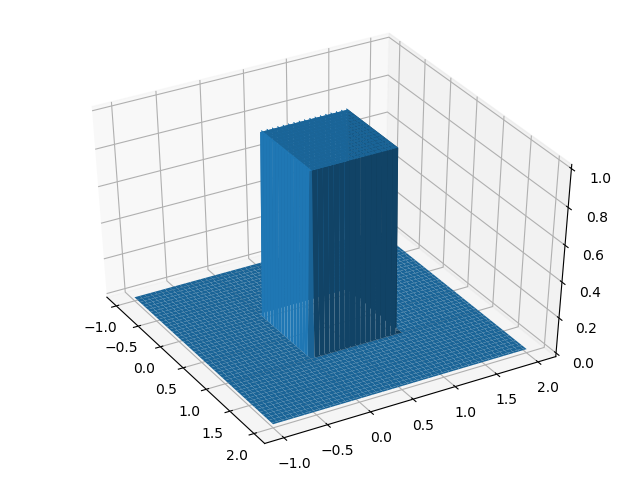
\includegraphics[scale=\myscale,scale=0.5]{figures/neurones-surface-1}
	\end{minipage}
\end{center}

%%%%%%%%%%%%%%%%%%%%%%%%%%%%%%%%%%%%%%%%%%%%%%%%%%%%%%%%%%%%%%%%%%%%%

\section{Gradient pour un réseau de neurones}

%--------------------------------------------------------------------
\subsection{Fonction associée à un réseau}
\label{ssec:foncres}

Pour un réseau de neurones $\mathcal{R}$ ayant $n$ entrées $(x_1,\ldots,x_n)$ et une seule sortie, nous associons une fonction : $F : \Rr^n \to \Rr$,  $(x_1,\ldots,x_n) \mapsto F(x_1,\ldots,x_n)$. La situation est en fait plus compliquée. Jusqu'ici les paramètres du réseau étaient donnés. \`A partir de maintenant les variables du problème ne seront plus les entrées mais les poids du réseau. 
Notons $a_1,\ldots,a_m$ ces poids (l'ensemble des coefficients et des biais). Si l'entrée est fixée et que les poids sont les variables du réseau alors on pourrait considérer que ce même réseau $\mathcal{R}$ définit la fonction 
$\widetilde F : \Rr^m \to \Rr$, $(a_1,\ldots,a_m) \mapsto \widetilde F(a_1,\ldots,a_m)$. 

\myfigure{0.6}{
	\tikzinput{fig-gradres-01}
}


Ce dont nous aurons besoin pour la suite et que nous allons calculer dans ce chapitre c'est le gradient de $\widetilde F$ par rapport aux poids $(a_1,\ldots,a_m)$, autrement dit, il s'agit de calculer :
$$\frac{\partial \widetilde F}{\partial a_j}.$$

Pour concilier les deux points de vue (entrées et poids), on dira qu'un réseau de neurones ayant des entrées $(x_1,\ldots,x_n)$ et des poids 
$(a_1,\ldots,a_m)$ définit la fonction :
$$\begin{array}{lccc}
	\widehat F : & \Rr^n             \times  \Rr^m & \longrightarrow & \Rr \\
	& (x_1,\ldots,x_n)  ,  (a_1,\ldots,a_m) & \longmapsto & \widehat F(x_1,\ldots,x_n,a_1,\ldots,a_m) \\
\end{array}$$

%\begin{remarque*}
Ce n'est pas tout à fait la fonction $\widetilde F$ dont on voudra calculer le gradient mais notre attention se portera sur une fonction d'erreur $E$ de la forme
$E = (\widetilde F-y_0)^2$, où $\widetilde F$ est la fonction définie ci-dessus correspondant à une certaine entrée et à la sortie $y_0$.
On calcule facilement les dérivées partielles de $E$ à partir de celles de $\widetilde F$ par la formule :
$$\frac{\partial E}{\partial a_j} = 2\frac{\partial \widetilde F}{\partial a_j}(\widetilde F-y_0).$$
Voir le chapitre \og{}Rétropropagation\fg{} pour plus de détails.
%\end{remarque*}


%--------------------------------------------------------------------
\subsection{Formule du gradient}

On considère la portion suivante d'un réseau de neurones :
\myfigure{1}{
	\tikzinput{fig-gradres-02}
}
On s'intéresse à une seule arête entrante du neurone central\couleurnb{ rouge}{}, celle qui porte le poids $a$.
\begin{itemize}
	\item $a$ et $b$ sont des poids,
	\item $f, g, h$ sont des fonctions d'activation,
	\item $f', g', h'$ sont leur dérivées,
	\item $F$ est la fonction associée au réseau complet.
\end{itemize}

Pour distinguer la fonction de sa valeur en un point, on notera $f$ la fonction et $f_\mystar$ la valeur de la fonction à la sortie du neurone correspondant.

Voici la formule pour calculer la dérivée partielle de $F$ par rapport au coefficient $a$, connaissant la dérivée partielle par rapport au coefficient $b$.
\mybox{$\displaystyle
	\frac{\partial F}{\partial a} = f_\mystar \cdot \frac{g'_\mystar}{g_\mystar} \cdot b \cdot \frac{\partial F}{\partial b}
	$} 
Voici un schéma pour retenir cette \og{}\trouer{formule du sourire}\fg{}\index{formule du sourire}:
on multiplie les coefficients $f_\mystar$, $g'_\mystar$, $b$ et la dérivée partielle par rapport à $b$ le long de l'arc et on divise par le coefficient $g_\mystar$ au bout du segment.
\myfigure{1.4}{
	\tikzinput{fig-gradres-03}
}
Il est à noter que dans la formule, seule l'arête portant le coefficient $a$ intervient, les autres arêtes entrantes n'interviennent pas (et ne sont pas représentées). 
Par contre, dans le cas de plusieurs arêtes sortantes il faut calculer la somme 
des formules précédentes sur chaque arête :
\mybox{$\displaystyle
	\frac{\partial F}{\partial a} = \sum_{i=1}^{\ell} f_\mystar \cdot \frac{g'_\mystar}{g_\mystar} \cdot b_{i} \cdot \frac{\partial F}{\partial b_i}
	$} 
Cette somme comporte autant de termes que d'arêtes sortantes (il n'y a pas à énumérer tous les chemins entre le sommet et la sortie comme auparavant dans la différentiation automatique).
\myfigure{1}{
	\tikzinput{fig-gradres-04}
}

\bigskip

Pour pouvoir calculer toutes les dérivées partielles, on procède par récurrence, en partant de la fin puis en revenant en arrière de proche en proche. 

\myfigure{1}{
	\tikzinput{fig-gradres-05}
}

Voici la formule d'initialisation associée aux coefficients en sortie de réseau, dite \og{}formule du demi-sourire\fg{} :
\mybox{$\displaystyle
	\frac{\partial F}{\partial a} = f_\mystar \cdot g'_\mystar
	$} 


\bigskip

Voici quelques situations particulières, mais qui sont simplement des applications de la formule du sourire.

\textbf{Formule à l'entrée.} On applique la formule du sourire avec $x$ à la place de $f$.
$$\frac{\partial F}{\partial a} = x \cdot \frac{g'_\mystar}{g_\mystar} \cdot b \cdot \frac{\partial F}{\partial b}$$ 
\myfigure{1}{
	\tikzinput{fig-gradres-06}
}

\textbf{Dérivée partielle par rapport aux variables d'entrées.}
On applique la formule du sourire en ajoutant des coefficients virtuels égaux à $1$ (la dérivée de $x$ par rapport à $x$ est $1$) :
$$\frac{\partial F}{\partial x} = \frac{b}{x} \cdot \frac{\partial F}{\partial b}$$
\myfigure{1}{
	\tikzinput{fig-gradres-07}
}


\textbf{Cas d'un biais.} On applique la formule du sourire en ajoutant un coefficient virtuel égal à $1$ :
$$\frac{\partial F}{\partial a} = \frac{g'_\mystar}{g_\mystar} \cdot b \cdot \frac{\partial F}{\partial b}$$ 
\myfigure{1}{
	\tikzinput{fig-gradres-08}
}


%\begin{remarque*}
%	\sauteligne
\begin{itemize}
	\item Ces formules ne sont pas valables lorsque $g_\star=0$. Nous verrons lors de la preuve de ces formules comment régler ce problème.
	
	\item Il faut s'habituer au jeu d'écriture un peu ambigu, comme on le fait pour une expression $y$ qui dépend de $x$. On peut noter cette expression $y(x)$ ou bien simplement $y$, cette dernière écriture peut désigner une fonction de $x$ ou bien la valeur prise en $x$. Par exemple dans la formule du sourire  $\frac{\partial F}{\partial a}$ et $ \frac{\partial F}{\partial b}$ sont en fait les valeurs des dérivées partielles et ne sont pas vraiment considérées comme des fonctions. Dans la pratique cela ne posera pas de problème car le but est de calculer les valeurs des dérivées partielles (et pas l'expression des fonctions dérivées partielles).
	
	\item De plus, les expressions sont dérivées par rapport à différentes variables. Par exemple, si une expression $F$ dépend de $y$, et l'expression $y$ dépend de $x$, alors on peut calculer  $\frac{\partial F}{\partial y}$, mais aussi $\frac{\partial F}{\partial x}$. 
	
	\item Enfin la fonction $F$ considérée ici dépend des variables d'entrée $x_i$ mais aussi des poids $a_j$, si on suivait le formalisme introduit en section \ref{ssec:foncres}, on devrait plutôt la noter  $\widehat F$.
\end{itemize}
%\end{remarque*}


%--------------------------------------------------------------------
\subsection{Premier exemple}

Voici un réseau très simple.
\myfigure{1}{
	\tikzinput{fig-gradres-09}
}
Avec :
\begin{itemize}
	\item une entrée $x$, une sortie $F(x)$,
	\item trois poids $a,b,c$,
	\item des fonctions d'activation (plutôt fantaisistes) $u \mapsto u^2$ et $v \mapsto \ln v$.
\end{itemize}
Nous avions l'habitude de considérer la fonction $x \mapsto F(x)$ mais dorénavant les poids sont de nouvelles variables, nous devons donc étudier la fonction 
$\widehat F$ introduite ci-dessus que nous noterons encore $F$ dans la suite :
$$F(x,a,b,c) = \ln\big( c (ax+b)^2 \big).$$
Nous souhaitons calculer les dérivées partielles de $F$ par rapport aux poids $a,b,c$. Nous ne souhaitons pas obtenir une formule générale mais juste la valeur exacte de ces dérivées partielles en un point précis. Nous choisissons l'exemple de 
$(x,a,b,c) = (2,3,4,5)$.
On récrit le réseau avec les valeurs des poids, les valeurs des fonctions et les valeurs des dérivées locales.
\myfigure{1}{
	\tikzinput{fig-gradres-10}
}


\textbf{Calcul de la dérivée partielle par rapport à $c$.}
On part de la sortie pour l'initialisation. On applique la formule du demi-sourire.
\myfigure{1}{
	\tikzinput{fig-gradres-11}
}
$$\frac{\partial F}{\partial c} = 100 \times \frac{1}{500} = \frac15.$$

\textbf{Calcul de la dérivée partielle par rapport à $a$.}
On applique la formule du sourire :
$$\frac{\partial F}{\partial a} = 2 \times \frac{20}{100} \times 5 \times \frac{\partial F}{\partial c}.$$
\myfigure{1}{
	\tikzinput{fig-gradres-12}
}
Mais on a déjà calculé $\frac{\partial F}{\partial c}=\frac15$ (entre accolades doubles), donc :
$$\frac{\partial F}{\partial a} = \frac25.$$

\textbf{Calcul de la dérivée partielle par rapport à $b$.}
On applique la formule du sourire (en posant $1$ pour le coefficient manquant):
$$\frac{\partial F}{\partial b} = 1 \times \frac{20}{100} \times 5 \times \frac{\partial F}{\partial c}.$$
\myfigure{1}{
	\tikzinput{fig-gradres-13}
}
Donc 
$$\frac{\partial F}{\partial b} = \frac15.$$

\textbf{Calcul de la dérivée partielle par rapport à $x$.}
On peut aussi calculer cette dérivée partielle, même si nous n'en aurons pas besoin dans les autres chapitres. 
$$\frac{\partial F}{\partial x} = 1 \times \frac{1}{2} \times 3 \times \frac{\partial F}{\partial a}.$$
\myfigure{1}{
	\tikzinput{fig-gradres-14}
}
donc 
$$\frac{\partial F}{\partial x} = \frac{3}{5}.$$

\textbf{Bilan.}
Ainsi $F(2,3,4,5)=\ln 500$ et on a calculé les dérivées partielles (entre doubles accolades) pour chacune des variables $x,a,b,c$.
\myfigure{1}{
	\tikzinput{fig-gradres-15}
}

\textbf{Vérification.}
On peut vérifier nos formules en calculant directement les dérivées partielles à partir de l'expression :
$$F(x,a,b,c) = \ln\big( c (ax+b)^2 \big).$$
Par exemple :
$$\frac{\partial F}{\partial a}(x,a,b,c) = \frac{2cx(ax+b)}{c(ax+b)^2} = \frac{2x}{ax+b}$$
et on a bien 
$$\frac{\partial F}{\partial a}(2,3,4,5) = \frac{4}{10} = \frac25.$$

%--------------------------------------------------------------------
\subsection{Second exemple}

Pour le réseau suivant, on associe comme précédemment une fonction $F$. 
\myfigure{1}{
	\tikzinput{fig-gradres-16}
}
On considère les poids $a,b,c,d$ comme des variables, la fonction $F : \Rr^5 \to \Rr$ s'écrit donc :
$$F(x,a,b,c,d) = \exp\big(c \cos(ax) + d\sin(bx)\big).$$

On va noter $u=ax$ et $v=bx$, ainsi $\cos u$ et $\sin v$ sont les sorties des deux premiers neurones. On note $w =c\cos u + d\sin v$. La sortie du troisième neurone (qui est aussi la valeur de $F$) est alors $\exp w$.

On part de la sortie pour l'initialisation. Il y a deux dérivées partielles à calculer.

\textbf{Calcul de la dérivée partielle par rapport à $c$.}
On applique la formule du demi-sourire :
$$\frac{\partial F}{\partial c} = \cos u \cdot \exp w.$$

\textbf{Calcul de la dérivée partielle par rapport à $d$.}
On applique de nouveau la formule du demi-sourire :
$$\frac{\partial F}{\partial d} = \sin v \cdot \exp w.$$

\textbf{Calcul de la dérivée partielle par rapport à $a$.}
On applique la formule du sourire :
$$\frac{\partial F}{\partial a} = x \cdot \frac{-\sin u}{\cos u} \cdot c \cdot  \frac{\partial F}{\partial c}$$
donc 
$$\frac{\partial F}{\partial a} = -x c \sin u \exp w.$$

\textbf{Calcul de la dérivée partielle par rapport à $b$.}
On applique la formule du sourire :
$$\frac{\partial F}{\partial b} = x \cdot \frac{\cos v}{\sin v} \cdot d \cdot  \frac{\partial F}{\partial d}$$
donc 
$$\frac{\partial F}{\partial b} = x d \cos v \exp w.$$

\textbf{Calcul de la dérivée partielle par rapport à $x$.}
Cette dérivée partielle s'obtient comme la somme de deux termes correspondant aux deux arêtes sortantes :
$$\frac{\partial F}{\partial x} = a \cdot \frac{1}{x} \cdot \frac{\partial F}{\partial a} \ + \  b \cdot \frac{1}{x} \cdot \frac{\partial F}{\partial b}$$
donc 
$$\frac{\partial F}{\partial x} = (-ac\sin u + bd\cos v) \exp w.$$

\textbf{Vérification.}
En effectuant les substitutions $u=ax$, $v=bx$ et $w =c\cos (ax) + d\sin (bx)$,
on retrouve les dérivées partielles attendues, par exemple
$$\frac{\partial F}{\partial x} = \big(-ac\sin (ax) + bd\cos (bx) \big) \exp \big(c\cos (ax) + d\sin (bx) \big).$$

%--------------------------------------------------------------------
\subsection{Preuve et formule générale}

\myfigure{1}{
	\tikzinput{fig-gradres-17}
}

\textbf{Préliminaires.}

\mybox{
	\begin{equation}
		\frac{\partial h}{\partial g} = b \cdot h'_\mystar
		\label{eq:grad:eq1}
	\end{equation}
}
Preuve : on a $h_\mystar = h(b g_\mystar)$, la formule s'obtient en dérivant $g \mapsto h(bg)$ par rapport à la variable $g$, avec 
$h'_\mystar = h'(b g_\mystar)$.

\mybox{
	\begin{equation}
		\frac{\partial g}{\partial a} = f_\mystar \cdot g'_\mystar
		\label{eq:grad:eq2}
	\end{equation}
}
Preuve : on a $g_\mystar = g(\cdots + a f_\mystar+\cdots)$, la formule s'obtient en dérivant $a \mapsto g(\cdots + a f +\cdots)$ par rapport à la variable $a$. On note $g'_\mystar = g'(\cdots + a f_\mystar+\cdots)$.

\mybox{
	\begin{equation}
		\frac{\partial h}{\partial b} = g_\mystar \cdot h'_\mystar
		\label{eq:grad:eq3}
	\end{equation}
}
Preuve : c'est la même formule que l'équation (\ref{eq:grad:eq2}) mais cette fois pour $b \mapsto h(b g)$ et $h'_\mystar = h'(b g_\mystar)$.

\bigskip
\textbf{Formule générale.}

\mybox{
	\begin{equation}
		\frac{\partial F}{\partial a} = \frac{\partial F}{\partial g} \cdot f_\mystar \cdot  g'_\mystar
		\label{eq:grad:eq4}
	\end{equation}
}

Preuve :
c'est la formule
$$\frac{\partial F}{\partial a} =  \frac{\partial F}{\partial g} \cdot \frac{\partial g}{\partial a}$$
(valable car $g$ est une fonction d'une seule variable) suivie de l'application de l'équation (\ref{eq:grad:eq2}).

\mybox{
	\begin{equation}
		\frac{\partial F}{\partial g} = \frac{\partial F}{\partial h} \cdot b \cdot  h'_\mystar
		\label{eq:grad:eq5}
	\end{equation}
}

Preuve :
c'est la formule
$$\frac{\partial F}{\partial g} =  \frac{\partial F}{\partial h} \cdot \frac{\partial h}{\partial g}$$
suivie de l'application de l'équation (\ref{eq:grad:eq1}).

Dans le cas d'un neurone de sortie on a :
\mybox{
	\begin{equation}
		\frac{\partial F}{\partial g} = 1
		\label{eq:grad:eq6}
	\end{equation}
}
car comme $g$ est la dernière fonction, on a $F_\mystar = g_\mystar$.

\bigskip
\textbf{Algorithme.}


\myfigure{1}{
	\tikzinput{fig-gradres-18}
}
Voici comment calculer toutes les dérivées partielles voulues (y compris dans le cas $g_\mystar=0$ qui avait été exclu dans la formule du sourire).
\begin{itemize}
	\item On part du neurone de sortie pour lequel on initialise le processus par la formule
	(\ref{eq:grad:eq6}) ce qui donne 
	$\frac{\partial F}{\partial g_n} = 1$.
	\item On procède par récurrence à rebours. On suppose que l'on a déjà calculé
	$\frac{\partial F}{\partial g_{i+1}}$
	On en déduit :
	$$\frac{\partial F}{\partial g_{i}} =  \frac{\partial F}{\partial g_{i+1}} \cdot a_{i+1} \cdot  g'_{i+1,\mystar}$$
	par la formule (\ref{eq:grad:eq5}).
	\item Cela permet de calculer les dérivées partielles par rapport aux poids à l'aide de la formule (\ref{eq:grad:eq4}) :
	$$\frac{\partial F}{\partial a_i} = \frac{\partial F}{\partial g_i} \cdot g_{i-1,\mystar} \cdot  g'_{i,\mystar}.$$
\end{itemize}



\bigskip
\textbf{Preuve de la formule du sourire.}

On va exprimer $\frac{\partial F}{\partial a}$ directement en fonction de $\frac{\partial F}{\partial b}$.

Par les équations (\ref{eq:grad:eq4}) et (\ref{eq:grad:eq5}), on a d'une part :
\begin{equation}
	\frac{\partial F}{\partial a} =   \frac{\partial F}{\partial h} \cdot b \cdot  h'_\mystar \cdot f_\mystar \cdot g'_\mystar
	\label{eq:grad:eq7}
\end{equation}
et d'autre part :
$$\frac{\partial F}{\partial b} =  \frac{\partial F}{\partial h} \cdot \frac{\partial h}{\partial b}.$$
Donc, en utilisant l'équation (\ref{eq:grad:eq3}), on obtient :
\begin{equation}
	\frac{\partial F}{\partial b} =   \frac{\partial F}{\partial h} \cdot g_\mystar \cdot  h'_\mystar.
	\label{eq:grad:eq8}
\end{equation}
Cette dernière équation permet de calculer $\frac{\partial F}{\partial h}$ en fonction $\frac{\partial F}{\partial b}$. Ainsi des équations (\ref{eq:grad:eq7}) et (\ref{eq:grad:eq8}), on obtient la formule du sourire :
$$\frac{\partial F}{\partial a} = f_\mystar \cdot \frac{g'_\mystar}{g_\mystar} \cdot b \cdot \frac{\partial F}{\partial b}.$$

Dans le cas de plusieurs arêtes sortantes, il s'agit de faire une somme comme on l'a déjà vu lors de la différentiation automatique.



%%%%%%%%%%%%%%%%%%%%%%%%%%%%%%%%%%%%%%%%%%%%%%%%%%%%%%%%%%%%%%%%%%%%%

\index{retropropagation@rétropropagation}
\index{descente de gradient!retropropagation@rétropropagation}

%%%%%%%%%%%%%%%%%%%%%%%%%%%%%%%%%%%%%%%%%%%%%%%%%%%%%%%%%%%%%%%%%%%%%
\section{Principe de la rétropropagation}

La rétropropagation, c'est la descente de gradient appliquée aux réseaux de neurones. Nous allons étudier des problèmes variés et analyser les solutions produites par des réseaux de neurones.
	
Voici un jeu de données : des ronds bleus et des carrés rouges.
Nous souhaitons trouver un modèle simple qui caractérise ces données.


\begin{center}
	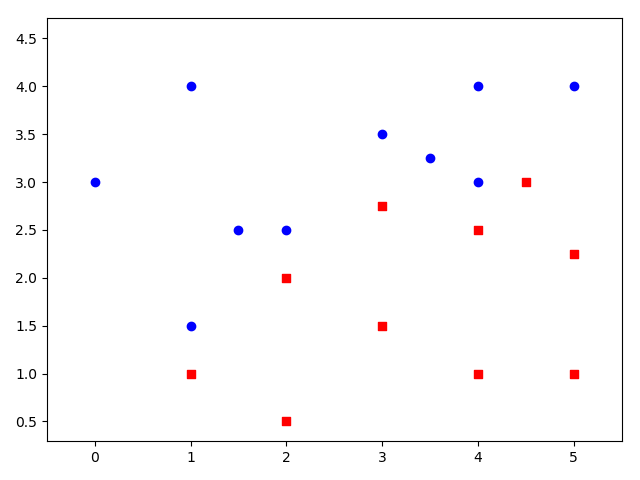
\includegraphics[scale=\myscale,scale=0.5]{figures/retro_01_a}
\end{center}

Plus exactement, nous souhaiterions pouvoir dire pour chaque point du plan s'il devrait être colorié en rouge ou bien en bleu et ceci pour des points qui ne sont pas dans les données de départ. De plus, nous voulons ne rien faire à la main, mais que la réponse soit calculée par la machine !

Nous allons revoir pas à pas l'utilisation d'un réseau de neurones pour résoudre un problème et traiterons en particulier l'exemple ci-dessus.

%--------------------------------------------------------------------
\subsection{Objectif du réseau}

\begin{itemize}
	\item Soit $\mathcal{R}$ un réseau de neurones. Celui-ci est défini par son architecture (le nombre de couches, le nombre de neurones par couche), les fonctions d'activation et l'ensemble $P = (a_1,a_2,\ldots)$ des poids de tous les neurones.
	
	\item \`A ce réseau $\mathcal{R}$ on associe une fonction $F : \Rr^n \to \Rr^p$ où $n$ est la dimension des entrées (de la première couche) et $p$ le nombre de neurones de la couche de sortie.
	Dans ce chapitre, nous supposerons qu'il n'y a qu'une seule sortie, c'est-à-dire $p=1$ et $F : \Rr^n \to \Rr$.
	
	\myfigure{0.8}{
		\tikzinput{fig_retro_04}
	} 
	
	
	\item On dispose de données $(X_i,z_i)$ (pour $i=1,\ldots,N$) où $X_i \in \Rr^n$ est une \trouer{entrée} (de la forme $X=(x_1,\ldots,x_n)$) et $z_i \in \Rr$ est la \trouer{sortie attendue} pour cette entrée.
	
	\item Le but est de trouver les poids du réseau afin que la fonction $F$ qui lui est associée vérifie :
	$$F(X_i) \simeq z_i \quad \text{pour tout} \quad i=1,\ldots,N.$$ 
	
	\item Pour mesurer précisément la performance de l'approximation, on définit une \trouer{fonction erreur} :
	$$E = \frac{1}N \sum_{i=1}^N E_i \qquad \text{ avec } \qquad \quad E_i = \big( F(X_i) - z_i \big)^2.$$
\end{itemize}


\begin{exemple}{}{}
	Nous traitons l'exemple donné en introduction.
	\begin{itemize}
		\item On décide de construire le réseau le plus simple possible : avec un seul neurone. Cela correspond à séparer les points du plan selon une droite.
		On choisit la fonction d'activation $\sigma$.
		La dimension de l'entrée est $2$ et celle la sortie est $1$.
		Il y a $3$ poids $(a,b,c)$ à calculer pour terminer le paramétrage du réseau.
		
		\myfigure{1.5}{
			\tikzinput{fig_retro_05}
		}   
		
		\item Pour chaque triplet de poids $(a,b,c)$ notre réseau définit une fonction $F : \Rr^2 \to \Rr$
		qui est en fait ici :
		$$F(x,y) = \sigma(ax+by+c)$$
		avec $\sigma(t) = \frac{1}{1+e^{-t}}$.
		
		
		
		\item Nos données sont les points rouges et bleus.
		Une entrée $X_i$ est donc constituée des coordonnées $(x_i,y_i)$ d'un point et la sortie attendue pour ce point est $z_i = 0$ (pour les points bleus) et $z_i = 1$ (pour les points rouges).
		Voici les coordonnées des ronds bleus (sortie attendue $z_i = 0$) :
		$$(0,3),\ (1,1.5),\ (1,4),\ (1.5,2.5),\ (2,2.5),\ (3,3.5),\ (3.5,3.25),\ (4,3),\ (4,4),\ (5,4)$$
		et des carrés rouges (sortie attendue $z_i = 1$) :
		$$(1,1),\ (2,0.5),\ (2,2),\ (3,1.5),\ (3,2.75),\ (4,1),\ (4,2.5),\ (4.5,3),\ (5,1),\ (5,2.25).$$  
		
		
		\item Comment définir les poids $(a,b,c)$ afin que $F(x_i,y_i) \simeq 0$ pour tous les ronds bleus et que $F(x_i,y_i)\simeq1$ pour tous les carrés rouges ? Si on sait trouver de tels poids alors on pourra colorier (presque) n'importe quel point $(x,y)$ du plan (et pas seulement nos ronds et nos carrés) : si $F(x,y) \simeq 0$, on coloriera le point en bleu, si par contre $F(x,y) \simeq 1$, on le coloriera en rouge.
		Plus précisément, la fonction $F$ (qui dépend de $\sigma$) a ses valeurs dans $[0,1]$ et prend la valeur $F(x,y)=\frac12$ exactement sur la droite $ax+by+c=0$. Ainsi, la fonction $F$ sépare le plan en deux demi-plans $\{ (x,y) \mid F(x,y)\le\frac12\}$ et $\{ (x,y) \mid F(x,y)\ge\frac12\}$ le long de la droite $ax+by+c=0$.
		
		\myfigure{0.7}{
			\tikzinput{fig_retro_06}
		}  
		\item L'erreur commise par la fonction $F$ associée aux poids $a,b,c$ est :
		$$E = E(a,b,c) = \frac{1}N \sum_{i=1}^N E_i(a,b,c)$$
		où $N$ est le nombre total des données (le nombre de ronds bleus plus le nombre de carrés rouges)
		et 
		$$E_i(a,b,c) = \big( F(x_i,y_i) - z_i \big)^2.$$
		On peut détailler un peu plus pour chaque type de point.
		En effet, pour un rond bleu la sortie attendue est $z_i=0$ donc $E_i(a,b,c) = \big( \sigma(a x_i + b y_i + c) - 0 \big)^2$, alors que pour un carré rouge la sortie attendue est $z_i=1$ donc $E_i(a,b,c) = \big( \sigma(a x_i + b y_i + c) - 1 \big)^2$.
		
	\end{itemize}
\end{exemple}


%--------------------------------------------------------------------
\subsection{Apprentissage}
L'apprentissage du réseau consiste à trouver les meilleurs poids en minimisant l'erreur par descente de gradient.

\begin{itemize}
	\item Pour trouver les poids $P = (a_1,a_2,\ldots)$ qui définissent le meilleur réseau $\mathcal{R}$ (autrement dit la meilleure fonction $F$),
	il suffit de minimiser l'erreur $E$, vue comme une fonction des poids $P = (a_1,a_2,\ldots)$. Pour cela on utilise la méthode de la descente de gradient.
	
	\item On part de poids initiaux $P_0 = (a_1,a_2,\ldots)$, par exemple choisis au hasard. On fixe un pas $\delta$.
	
	\item On construit par itérations des poids $P_k$ selon la formule de récurrence :
	$$P_{k+1} = P_k - \delta \grad E(P_k).$$
	\`A chaque itération, l'erreur $E(P_k)$ diminue.
	On s'arrête au bout d'un nombre d'itérations fixé à l'avance.
	
	\item Pour calculer le gradient $\grad E = \frac 1N \sum_{i=1}^N \grad E_i$, il faut  
	calculer chacun des $\grad E_i$, c'est-à-dire les dérivées partielles par rapport à chacun des poids $a_j$ selon la formule :
	$$\frac{\partial E_i}{\partial a_j}(X_i) = 2 \frac{\partial F}{\partial a_j}(X_i)  \big( F(X_i) - z_i \big).$$
\end{itemize}  


\begin{exemple}{}{}
	Poursuivons l'étude de notre exemple.
	\begin{itemize}
		\item La fonction $E(a,b,c)$ dépend des poids $a,b,c$.
		
		\item On part de poids initiaux $P_0 = (a_0,b_0,c_0)$, par exemple $P_0 = (0,1,-2)$ qui correspond à séparer le plan selon la droite horizontale $y=2$. 
		On fixe le pas $\delta = 1$.
		
		\item On calcule l'erreur locale pour la donnée numéro $i$ :
		$$E_i(a,b,c) = \big( F(x_i,y_i) - z_i \big)^2 = \big( \sigma(ax_i + by_i + c) - z_i \big)^2$$
		avec $z_i = 0$ ou $z_i=1$.
		
		\item Comme $\sigma'(x)= \sigma(x)(1-\sigma(x))$, alors, en notant $\sigma_i = \sigma(ax_i+by_i+c)$, on a :
		$$\frac{\partial E_i}{\partial a}(a,b,c) = 2 x_i  \sigma_i(1-\sigma_i)(\sigma_i - z_i)$$
		$$\frac{\partial E_i}{\partial b}(a,b,c) = 2 y_i \sigma_i(1-\sigma_i)(\sigma_i - z_i)$$
		$$\frac{\partial E_i}{\partial c}(a,b,c) = 2 \sigma_i(1-\sigma_i)(\sigma_i - z_i)$$ 
		et par suite 
		{\small
			$$\grad E_i(a,b,c) = \left(\frac{\partial E_i}{\partial a}(a,b,c), \frac{\partial E_i}{\partial b}(a,b,c), \frac{\partial E_i}{\partial c}(a,b,c) \right)
			\qquad \text{ et  } \qquad 
			\grad E(a,b,c) = \frac 1N \sum_{i=1}^N \grad E_i.$$
		}
		
		\item On part de $P_0 = (0,1,-2)$, on calcule $\grad E(P_0) = (-0.077, 0.192, 0.005)$. On obtient le poids suivant par $P_1 = P_0 - \delta \grad E(P_0) = (0.077,    0.807,    -2.005)$ (avec $\delta = 1$).   
		
		\item On continue avec la formule de récurrence $P_{k+1} = P_k - \delta \grad E(P_k)$ pour obtenir les poids suivants :
		
		$$
		\begin{array}{c|c|c|c}
			k & P_k = (a_k,b_k,c_k) & \grad E(a_k,b_k,c_k) & E(a_k,b_k,c_k) \\ \hline  
			0 & (0, 1, -2)                   & (-0.077, 0.192, 0.005)       & 0.450 \\
			1 & (0.077,    0.807,    -2.005) & (-0.072,   0.213,   0.0069 ) & 0.404 \\
			2 & (0.149,    0.593,    -2.012) & (-0.094,   0.188,  -0.0062 ) & 0.355 \\
			3 & (0.244,    3 0.4,    -2.006) & (-0.120,   0.137,  -0.0237 ) & 0.313 \\
			4 & (0.364,    0.267,    -1.982) & (-0.090,   0.126,  -0.0240 ) & 0.282 \\
			5 & (0.455,    0.140,    -1.958) & (-0.073,   0.109,  -0.0263 ) & 0.259 \\
			6 & (0.528,    0.031,    -1.932) & (-0.059,   0.095,  -0.0278 ) & 0.242 \\
			7 & (0.588,   -0.063,    -1.904) & (-0.051,   0.083,  -0.0290 ) & 0.229 \\
			8 & (0.639,   -0.146,    -1.875) & (-0.044,   0.074,  -0.0297 ) & 0.219 \\
			9 & (0.684,   -0.221,    -1.845) & (-0.040,   0.067,  -0.0302 ) & 0.211 \\
			10 & (0.72,   -0.288,    -1.815) & (-0.036,   0.061,  -0.0305 ) & 0.205 \\
			\cdots & & & \\
			100 & (1.328 -1.828, 0.333) & (-0.00037, 0.00646, -0.01780) & 0.103 \\
			\cdots & & & \\
			1000 & (2.032, -3.860, 3.703) & (-0.00034, 0.00073, -0.00086) & 0.071 \\  
		\end{array}
		$$  
		
		Au bout de $k=1000$ itérations, on obtient les poids  $P_{1000} =(2.032, -3.860, 3.703)$. Le gradient est devenu très petit, ce qui signifie ici que l'on est proche d'un minimum. De plus, l'erreur ne diminue presque plus lors des itérations suivantes, nous avons atteint le minimum recherché. (Attention, l'erreur est très petite, mais ne tend pas vers $0$.)
		
		
		
		\item La droite $ax+by+c=0$ qui sépare le plan en deux demi-plans $\{ (x,y) \mid F(x,y)\le\frac12\}$ et $\{ (x,y) \mid F(x,y)\ge\frac12\}$ évolue à chaque itération pour finir par séparer le mieux possible les ronds des carrés.
		
		\begin{center}
			\begin{minipage}{0.45\textwidth}
				\center \textbf{$k=0$ (initialisation)} 
				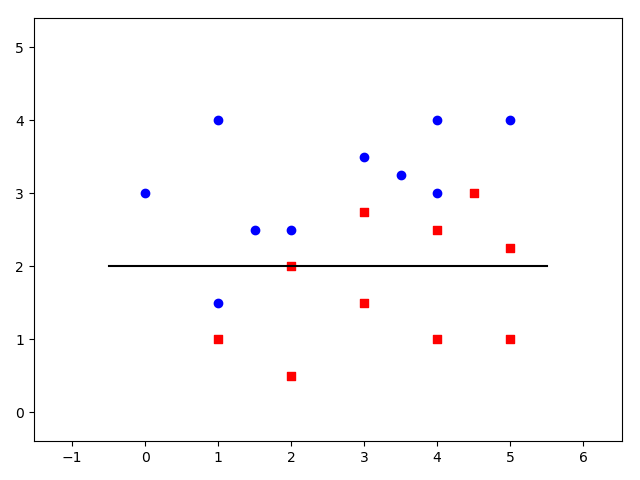
\includegraphics[scale=\myscale,scale=0.4]{figures/retro_01_b}
			\end{minipage}
			\begin{minipage}{0.45\textwidth}
				\center \textbf{$k=1$ (première itération)}
				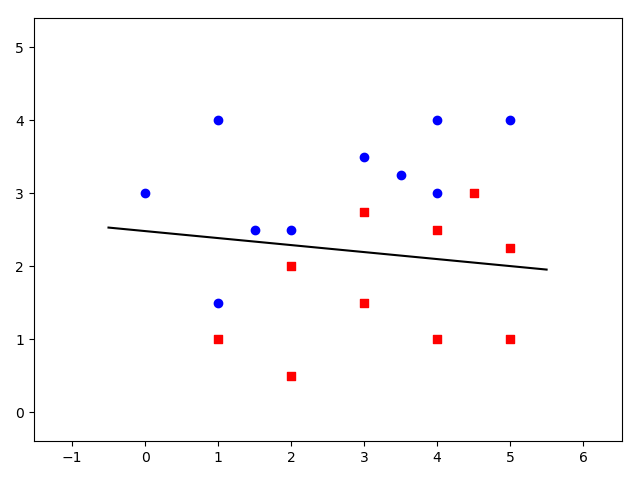
\includegraphics[scale=\myscale,scale=0.4]{figures/retro_01_c}
			\end{minipage}
			
			\begin{minipage}{0.45\textwidth}
				\center \textbf{$k=100$}
				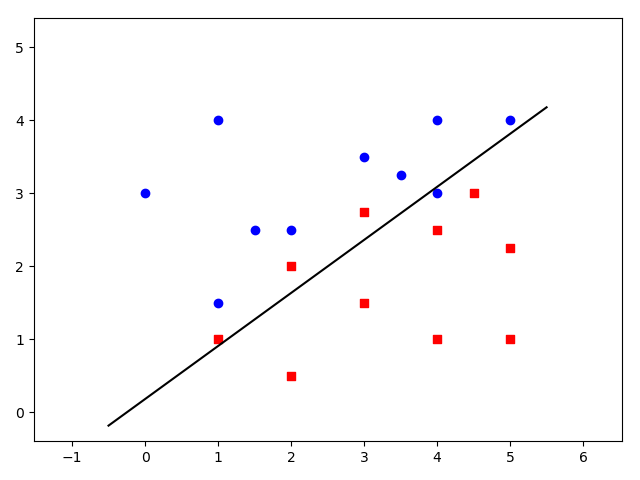
\includegraphics[scale=\myscale,scale=0.4]{figures/retro_01_d}
			\end{minipage}
			\begin{minipage}{0.45\textwidth}
				\center \textbf{$k=1000$}
				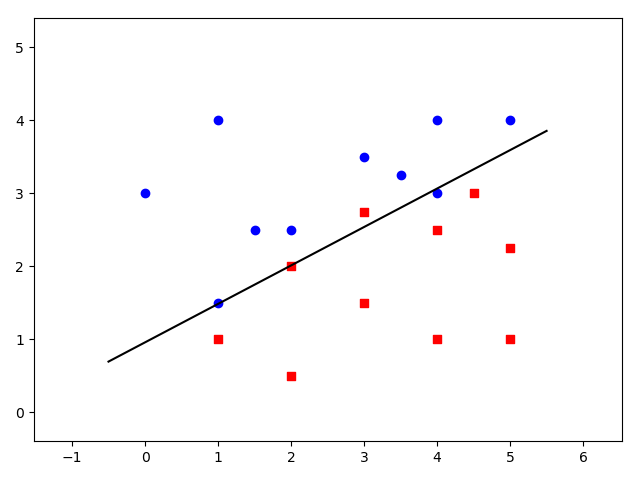
\includegraphics[scale=\myscale,scale=0.4]{figures/retro_01_e}
			\end{minipage}
		\end{center}
		
	\end{itemize}  
\end{exemple}


%--------------------------------------------------------------------
\subsection{Prédiction}

La conception d'un réseau de neurones est réalisée en modélisant au mieux les données injectées. Mais l'objectif réel est de faire des prédictions pour de nouvelles valeurs, jamais rencontrées auparavant.
La descente de gradient produit un ensemble de poids $P$ qui définit complètement notre réseau $\mathcal{R}$.
Nous obtenons donc une fonction $F : \Rr^n \to \Rr^p$, construite de sorte que $F(X_i) \simeq z_i$.
Nous pouvons évaluer cette fonction pour tout $X \in \Rr^n$, même pour des $X$ différents des $X_i$.


\begin{exemple}{}{}
	Dans notre exemple, nous avons obtenu par la descente de gradient les poids $P_{1000} = (a,b,c) = (2.032, -3.860, 3.703)$.
	Notre neurone $\mathcal{R}$ est maintenant opérationnel et définit ici la fonction 
	$$F(x,y) = \sigma(ax+by+c).$$
	
	\begin{center}
		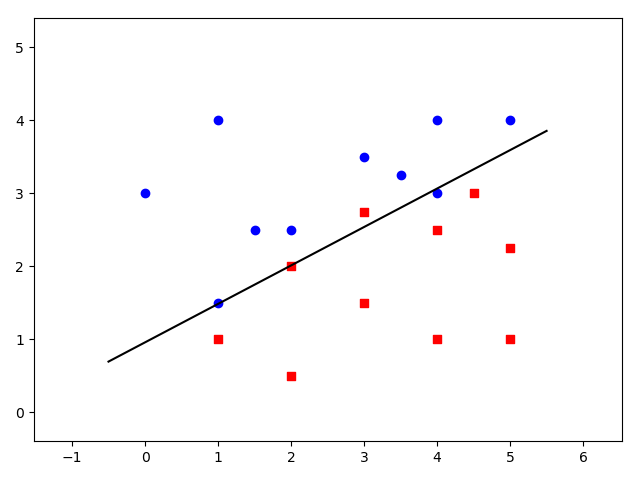
\includegraphics[scale=\myscale,scale=0.45]{figures/retro_01_e}
	\end{center}
	
	On souhaitait avoir $F(x_i,y_i)=0$ pour les ronds bleus et $F(x_i,y_i)=1$ pour les carrés rouges.
	Dans la pratique, on obtient des valeurs approchées, par exemple $F(0,3)=0.0003$ pour le rond bleu en $(0,3)$ et $F(1,1)=0.86$ pour le carré rouge en $(1,1)$.
	
	Notre fonction $F$ ne modélise pas parfaitement toutes nos données. Par exemple, pour le rond bleu en $(4,3)$ on a $F(4,3) = 0.56$ alors qu'on voudrait une valeur proche de $0$ et de même pour le carré rouge en $(3,2.75)$ on a $F(3,2.75) = 0.30$ alors qu'on voudrait une valeur proche de $1$. 
	
	Mais l'intérêt principal de $F$ est d'être définie pour tous les points du plan, ceci permet d'attribuer une couleur à chaque point $(x,y) \in \Rr^2$ selon la convention : bleu si $F(x,y)\simeq 0$, rouge si $F(x,y) \simeq 1$. Il y a bien sûr une \og{}zone grise\fg{} entre les zones rouge et bleue.
	
	Par exemple, $F(2,3) = 0.02$ donc $(2,3)$ mérite d'être colorié en bleu, $F(2,1) = 0.98$ donc $(2,1)$ mérite d'être colorié en rouge.
	La frontière en laquelle $F$ vaut $\frac12$ est la droite d'équation $ax+by+c=0$.
	
	Voici les niveaux de $F$ dans le plan (à gauche) et le graphe de $F$ dans l'espace (à droite).
	\begin{center}
		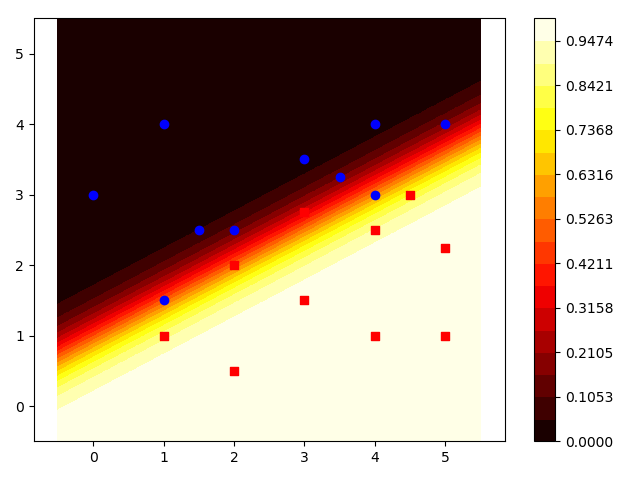
\includegraphics[scale=\myscale,scale=0.4]{figures/retro_01_g} \qquad
		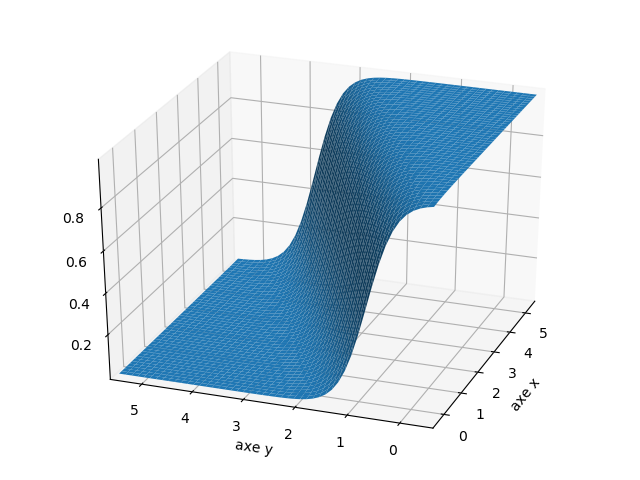
\includegraphics[scale=\myscale,scale=0.5]{figures/retro_01_f}
	\end{center}
	
	
	Nous avons choisi un réseau avec un seul neurone, la fonction $F$ est donc nécessairement très simple (quels que soient les poids) et ne peut pas \og{}coller\fg{} parfaitement aux données. 
	Nous avons séparé au mieux les ronds bleus des carrés rouges par une droite. Avec un réseau plus complexe, et donc une frontière plus compliquée, nous aurions pu \og{}coller\fg{} parfaitement aux données. Cependant est-ce vraiment ce que nous souhaitons faire ? Pour les données de notre exemple, avoir une séparation par une droite semble raisonnable. Peut-être que les points transfuges sont des erreurs de mesure.
	
\end{exemple}

%%%%%%%%%%%%%%%%%%%%%%%%%%%%%%%%%%%%%%%%%%%%%%%%%%%%%%%%%%%%%%%%%%%%%

\section{Exemples}

%--------------------------------------------------------------------
\subsection{Le \og{}ou exclusif\fg{}}

Rappelons le problème du \og{}ou exclusif\fg{}\index{ou exclusif} : il s'agit de trouver un réseau de neurones dont la fonction associée $F$ vaut $1$ en $(0,1)$ et $(1,0)$ (les carrés rouges) et vaut $0$ en $(0,0)$ et $(1,1)$ (les rond bleus).

\myfigure{1}{
	\tikzinput{fig_retro_01}
}

\textbf{Réseau.}

On a vu qu'il existe une solution avec un réseau à deux couches de fonction d'activation la fonction de Heaviside (voir le chapitre \og{}Réseau de neurones\fg{}).
On cherche à l'aide de la machine quels poids pourraient convenir avec la fonction d'activation sigmoïde :
\myfigure{1}{
	\tikzinput{fig_retro_02}
}

Il y a donc $9$ coefficients à déterminer.
La fonction d'erreur est :
$$E = (F(0,0) - 0)^2 + (F(1,1) - 0)^2 + (F(0,1)-1)^2 + (F(1,0) - 1)^2$$
sachant que $F$ et donc l'erreur $E$ dépendent des coefficients $a_1,\ldots,a_9$.
Il s'agit de trouver ceux qui rendent l'erreur $E$ minimale.

\bigskip

\textbf{Descente de gradient.}
On applique la méthode de la descente de gradient à la fonction $E$ pour les variables $(a_1,\ldots,a_9)$.
On utilise la descente de gradient classique avec un pas $\delta = 1$. 
Le choix des poids initiaux est déterminant pour les résultats.
On choisit comme poids de départ :
$$P_0 = (a_1,\ldots,a_9) = (1.0, 2.0, -3.0, -3.0, -2.0, 1.0, 1.0, 1.0, -1.0).$$


L'erreur initiale vaut $E(P_0) = 0.2961$.
Le gradient $\grad E(P_0)$ vaut 
$$(0.00349, -0.00303, -0.00832, -0.00696, -0.01350, -0.01047, -0.00324, 0.01258, -0.04671).$$
Avec $\delta = 1$, la première itération modifie un petit peu les coefficients :
$$P_1 = (0.9965, 2.0030, -2.9916, -2.9930, -1.9864, 1.0104, 1.0032, 0.9874, -0.9532),$$
l'erreur a légèrement diminué et vaut maintenant $E(P_1) = 0.2935$.
La seconde itération donne :
$$P_2 = (0.9925, 2.0055, -2.9839, -2.9860, -1.9731, 1.0206, 1.0053, 0.9738, -0.9105)$$
et l'erreur vaut maintenant $E(P_2) = 0.2911$.

Au bout de $1000$ itérations :
$$P_{1000} = (3.5623, 3.5675, -5.5344, -5.3682, -5.3935, 1.8403, -6.3234, -6.3801, 3.1216)$$
et l'erreur vaut maintenant $E(P_{1000}) = 0.0097$.

\bigskip

\textbf{Validation et prédiction.}
Au bout de $1000$ itérations notre réseau de neurones est assez performant.
La fonction $F(x,y)$ obtenue vérifie :
$$F(0,0) = 0.08, \qquad F(1,1) = 0.10, \qquad F(1,0) = 0.89,  \qquad F(0,1) = 0.89.$$

Les ronds bleus sont donc clairement séparés des carrés rouges par les valeurs de $F$.

Quelle couleur est-il naturel d'associer au points $(0.2,0.9)$ ?
On calcule $F(0.2,0.9) = 0.87$ qui est assez proche de $1$, il est donc naturel de le colorier en rouge.

\bigskip

\textbf{Visualisation graphique.}
Voici deux représentations graphiques de la fonctions $F$ obtenue. À gauche par les lignes de niveau dans le plan et à droite par son graphe dans l'espace.
La fonction $F$ prend des valeurs proches de $1$ autour de la droite passant par $(1,0)$ et $(0,1)$
et se rapproche de $0$ partout ailleurs. 
\begin{center}
	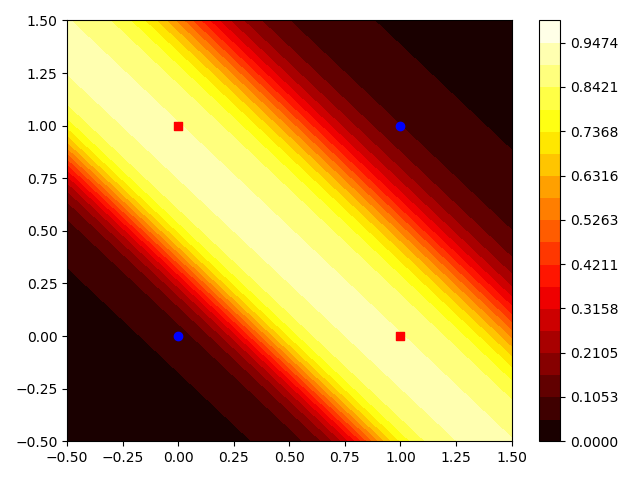
\includegraphics[scale=\myscale,scale=0.4]{figures/retro_02_a} \qquad
	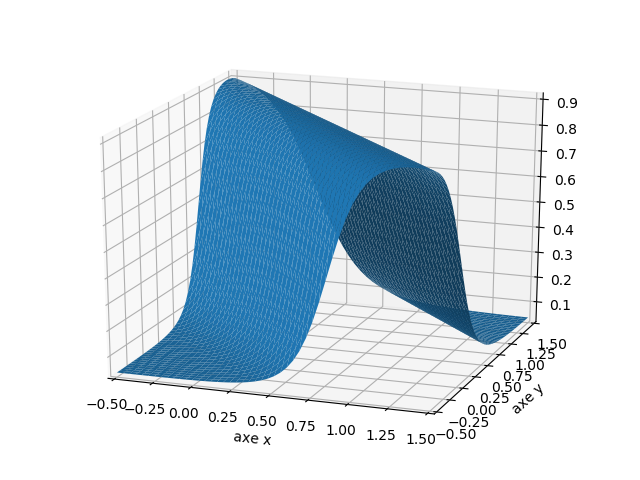
\includegraphics[scale=\myscale,scale=0.5]{figures/retro_02_b}
\end{center}

\bigskip

\textbf{Analyse.}
Voici l'évolution de l'erreur en fonction du nombre d'itérations. L'erreur décroît au fil des itérations : c'est le principe de la descente de gradient !
\begin{center}
	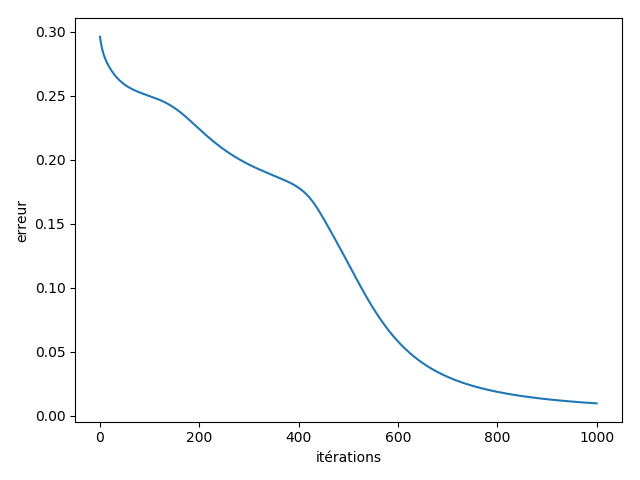
\includegraphics[scale=\myscale,scale=0.5]{figures/retro_02_c}
\end{center}


Comparer les poids obtenus avec ceux du \og{}ou exclusif\fg{} définis dans le chapitre \og{}Réseau de neurones\fg{}.

%--------------------------------------------------------------------
\subsection{Le perceptron et la règle de Hebb}

\index{perceptron}
\index{regle de Hebb@règle de Hebb}

Nous revenons sur l'exemple historique du cas d'un seul neurone (sans biais). Que donne la rétropropagation dans ce cas très simple ?

\myfigure{0.5}{
	\tikzinput{fig_retro_08}
}

Nous souhaitons une fonction d'activation du type marche Heaviside, qui renvoie $0$ ou $1$, mais pour la descente du gradient nous avons besoin d'une dérivée non nulle. Nous allons imaginer qu'il existe une fonction marche de Heaviside virtuelle $\widetilde H$ telle que
$$\widetilde H(x) = 0 \quad \text{si $x <0$} \qquad \widetilde H(x)=1 \quad \text{si $x\ge0$} \quad \text{ et } \quad \widetilde H'(x) = 1 \quad \text{pour tout $x\in \Rr$}.$$
Il est clair qu'une telle fonction n'existe pas (car la dérivée d'une fonction constante par morceaux est toujours nulle) mais faisons comme si c'était le cas.

Ce neurone définit une fonction $F$ telle que $F(x_1,\ldots,x_n) = \widetilde H(a_1x_1+\cdots+a_nx_n)$.
Comme d'habitude, nous avons des données $(X_i,z_i)$, ici $z_i=0$ ou bien $z_i=1$. Il s'agit de trouver les poids 
$(a_1,\ldots,a_n)$ tels que $F(X_i) \simeq z_i$.
L'erreur locale est donnée par $E_i = \big( F(X_i) - z_i \big)^2$.

La descente de gradient (stochastique) pour la donnée $i$ s'écrit : 
$$P_{k+1} = P_k - \delta \grad E_i(P_k).$$
On a : 
$$\frac{\partial E_i}{\partial a_j}(X_i) = 2 \frac{\partial F}{\partial a_j}(X_i)  \big( F(X_i) - z_i \big).$$
Mais $\frac{\partial F}{\partial a_j}(X_i) = x_j$ car $\widetilde H'(x)=1$ et comme
$F(X_i)$ et $z_i$ valent $0$ ou $1$, alors 
$\frac{\partial E_i}{\partial a_j}(X_i)$ vaut $\pm 2x_j$ ou $0$. Autrement dit, 
$\grad E_i = 2\epsilon(x_1,\ldots,x_n) = 2\epsilon X_i$ avec $\epsilon = 0$, $1$ ou $-1$.

\bigskip

Nous avons ainsi obtenu la \trouer{règle de Hebb}, qui est en fait l'ancêtre de la rétropropagation.

\textbf{Règle de Hebb.}
\begin{itemize}
	\item On fixe un pas $\delta>0$. 
	\item On part d'un poids $P_0$ (choisi au hasard par exemple).
	\item On calcule par récurrence les poids $P_k$ en parcourant la liste $(X_i,y_i)$ et en distinguant les cas suivants :
	\begin{itemize}
		\item si la sortie prédite $F(X_i)$ vaut la sortie attendue $z_i$ alors on ne change rien :
		$$P_{k+1} = P_k,$$
		\item si la sortie prédite $F(X_i)$ vaut $1$ alors que la sortie attendue $z_i$ vaut $0$ alors :
		$$P_{k+1} = P_k - 2\delta X_i,$$
		\item si la sortie prédite $F(X_i)$ vaut $0$ alors que la sortie attendue $z_i$ vaut $1$ alors :
		$$P_{k+1} = P_k + 2\delta X_i.$$  
	\end{itemize}
	
	\item Une fois toutes les données $(X_i,z_i)$ utilisées, on recommence depuis la première donnée.
	
	\item On s'arrête au bout d'un nombre d'itérations fixé à l'avance.
	\item Le dernier poids obtenu $P_k = (a_1,\ldots,a_n)$ définit le perceptron et la fonction associée qui répond au problème est :
	$F(x_1,\ldots,x_n)=1$ si $a_1x_1+\cdots+a_nx_n\ge0$ et $F(x_1,\ldots,x_n)=0$ sinon.
	
\end{itemize}



%--------------------------------------------------------------------
\subsection{Une fonction marche}

Nous avons vu dans le chapitre  \og{}Réseau de neurones\fg{} qu'il est facile de réaliser des fonctions \og{}marche\fg{} à l'aide d'un réseau simple et de la fonction de Heaviside.
Nous souhaitons construire un réseau de neurones dont la fonction $x \mapsto F(x)$ réalise au mieux les contraintes suivantes : $F(x)$ vaut $0$ sur $[0,2]$, puis vaut $1$ sur $[3,5]$ et de nouveau vaut
$0$ sur $[6,8]$ (il y a une certaine liberté sur $[2,3]$ et $[5,6]$).

\myfigure{0.7}{
	\tikzinput{fig_retro_07}
}

\bigskip

\textbf{Données.}
On décide de placer $10$ ronds bleus espacés régulièrement sur $[0,2]$, la même chose sur 
$[6,8]$, là où la fonction doit être nulle, et également $10$ carrés rouges espacés régulièrement sur $[3,5]$ là où la fonction doit valoir $1$. Ces points fournissent donc les $N=30$ données d'apprentissage. 

\begin{center}
	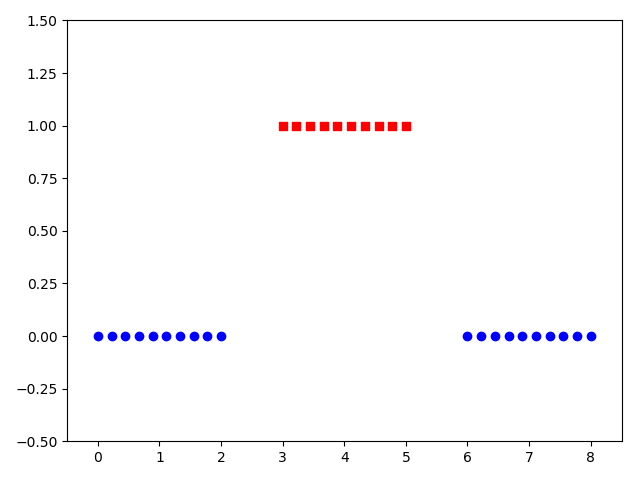
\includegraphics[scale=\myscale,scale=0.4]{figures/retro_03_a}
\end{center}

\bigskip

\textbf{Réseau.}
On décide d'utiliser un réseau avec deux neurones sur la couche d'entrée et un neurone sur la couche de sortie, tous utilisant la fonction d'activation $\sigma$.

\myfigure{1}{
	\tikzinput{fig_retro_09}
}

Il y a $7$ coefficients à déterminer.
La fonction d'erreur $E$ est la somme des $(F(x_i)-0)^2$ pour les $x_i$ abscisses des ronds bleus et des $(F(x_i)-1)^2$ pour les $x_i$ abscisses des carrés rouges.

\bigskip

\textbf{Descente de gradient.}
On applique la descente de gradient à la fonction $E$ de variables $(a_1,\ldots,a_7)$ pour un pas $\delta = 1$ et un choix arbitraire de poids initiaux :
$$P_0 = (a_1,\ldots,a_7) = (0.0, 1.0, 0.0, -1.0, 1.0, 1.0, -1.0).$$

Au bout de $5000$ itérations, on obtient les poids :
$$P_{5000} = (a_1,\ldots,a_7) = (-2.0142, 10.9964, 3.0543, -7.7086, 8.2334, 7.8735, -11.9037).$$


Voici l'évolution de l'erreur en fonction du nombre d'itérations.
\begin{center}
	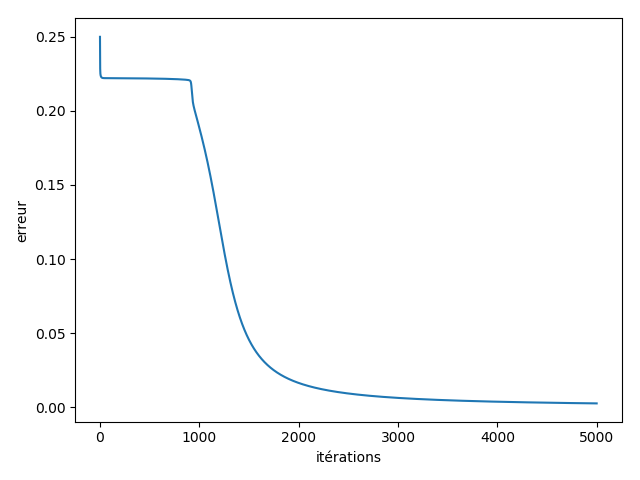
\includegraphics[scale=\myscale,scale=0.5]{figures/retro_03_f}
\end{center}


\bigskip

\textbf{Visualisation graphique.}

Voici le graphe de la fonction $x \mapsto F(x)$ au bout de différents nombres d'itérations.

\begin{center}
	\begin{minipage}{0.45\textwidth}
		\center \textbf{$k=0$ (initialisation)} 
		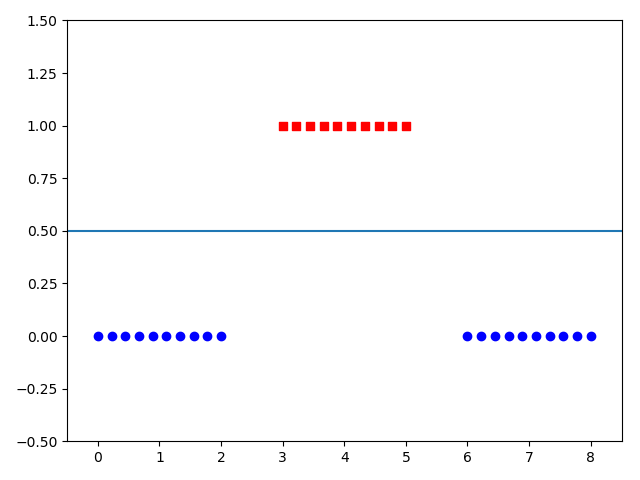
\includegraphics[scale=\myscale,scale=0.45]{figures/retro_03_b}
	\end{minipage}
	\begin{minipage}{0.45\textwidth}
		\center \textbf{$k=1000$}
		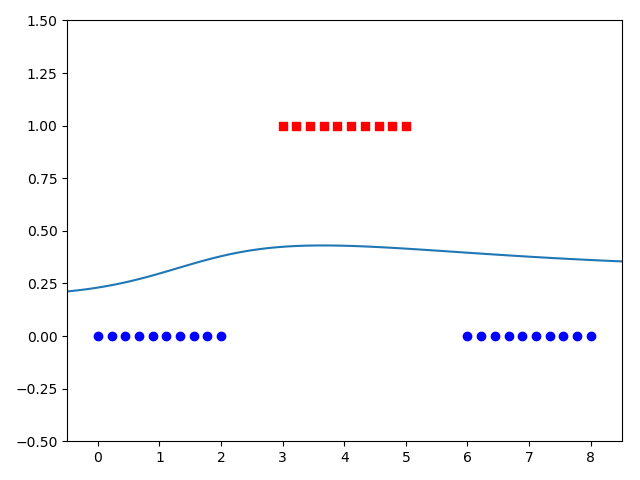
\includegraphics[scale=\myscale,scale=0.45]{figures/retro_03_c}
	\end{minipage}
	
	\begin{minipage}{0.45\textwidth}
		\center \textbf{$k=2000$}
		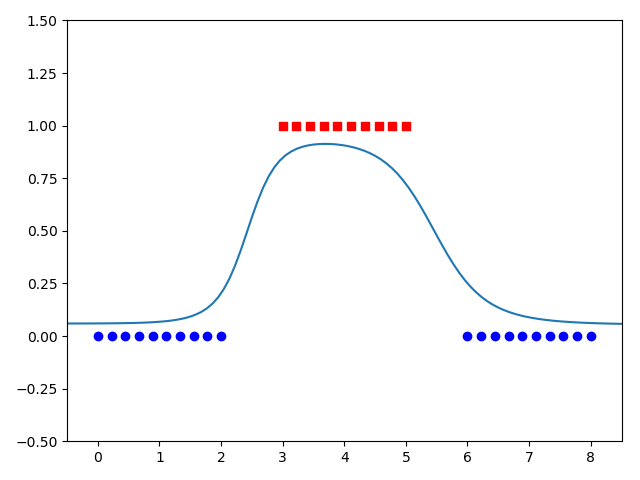
\includegraphics[scale=\myscale,scale=0.45]{figures/retro_03_d}
	\end{minipage}
	\begin{minipage}{0.45\textwidth}
		\center \textbf{$k=5000$}
		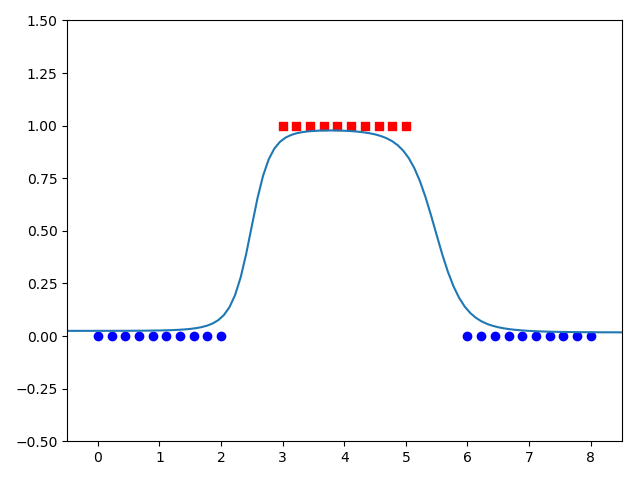
\includegraphics[scale=\myscale,scale=0.45]{figures/retro_03_e}
	\end{minipage}
\end{center}


%--------------------------------------------------------------------
\subsection{Plus de neurones}

Le but est ici de trouver un réseau de neurones qui distingue deux zones compliquées du plan : la zone bleue et la zone rouge.

\myfigure{1}{
	\tikzinput{fig_retro_10d}
}



Voici comme sont construites ces zones : on part d'une lemniscate de Bernoulli d'équation $(x^2+y^2)^2 = 4(x^2-y^2)$ et d'une ellipse d'équation
$(x-\frac12)^2 + 4(y-\frac13)^2=2$. 

\begin{center}
	\begin{minipage}{0.31\textwidth}
		\myfigure{0.47}{
			\tikzinput{fig_retro_10a}
		}
	\end{minipage}
	\quad
	\begin{minipage}{0.31\textwidth}
		\myfigure{0.47}{
			\tikzinput{fig_retro_10b}
		}
		
	\end{minipage}
	\quad
	\begin{minipage}{0.31\textwidth}
		\myfigure{0.47}{
			\tikzinput{fig_retro_10c}
		}
	\end{minipage}
\end{center}


L'union de ces deux courbes a pour équation :
$$f(x,y) = \big( (x^2+y^2)^2 - 4(x^2-y^2) \big)  \cdot \big((x-\tfrac12)^2 + 4(y-\tfrac13)^2 - 2 \big) = 0.$$
La zone rouge correspond aux points de coordonnées $(x,y)$ pour lesquels $f(x,y) \le 0$ et la zone bleue à $f(x,y) > 0$. Nous allons limiter notre étude à une zone rectangulaire. Le rectangle est choisi de sorte que l'aire bleue et l'aire rouge soient à peu près égales.

\textbf{Objectifs.} 
On oublie maintenant la fonction $f$ et on ne retient que quelques points rouges et quelques points bleus. On cherche un réseau et une fonction $F$ telle que $F(x,y) \simeq 1$ pour les points rouges et $F(x,y) \simeq 0$ pour les points bleus.

\textbf{Données.} 
On divise notre rectangle en une grille de $n \times n$ points. Les exemples ci-dessous sont calculés pour $n=200$. Nous avons donc $40\,000$ points $(x,y)$, repartis (à peu près) équitablement entre rouge ($z=1$) et bleu ($z=0$).

\textbf{Architecture.}
On décide de concevoir un réseau à $4$ couches, avec le même nombre $p$ de neurones par couche pour les trois premières couches et un seul neurone sur la couche de sortie. La fonction d'activation choisie pour tous les neurones est ReLU .
Voici une illustration de la configuration pour $p=3$.

\myfigure{0.8}{
	\tikzinput{fig_retro_11}
}


\textbf{Poids.} 
On calcule les poids avec une méthode de descente de gradient stochastique.
Les poids initiaux sont choisis aléatoirement, le nombre d'itérations est suffisamment grand.
Le réseau obtenu après calculs fournit donc une fonction $F$.
On colorie en rouge les points pour lesquels $F(x,y) \simeq 1$ (en fait, là où $F(x,y)\ge \frac12$) et en bleu les points pour lesquels $F(x,y) \simeq 0$ (en fait, là où $F(x,y)< \frac12$). On regarde si le résultat obtenu est proche de la situation envisagée.
On présente ici quelques résultats typiques intéressants (les résultats pouvant varier selon le choix aléatoire des poids initiaux).

\begin{center}
	\begin{minipage}{0.45\textwidth}
		\center {$p=3$, $10$ neurones, $37$ poids} 
		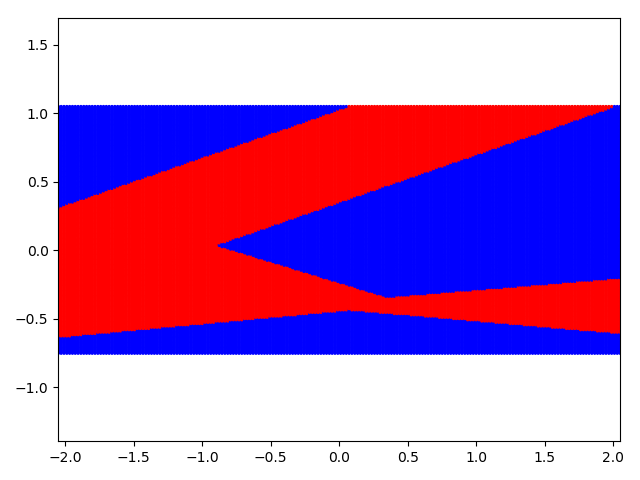
\includegraphics[scale=\myscale,scale=0.45]{figures/retro_05_p=3}
	\end{minipage}
	\begin{minipage}{0.45\textwidth}
		\center {$p=5$, $16$ neurones, $81$ poids}
		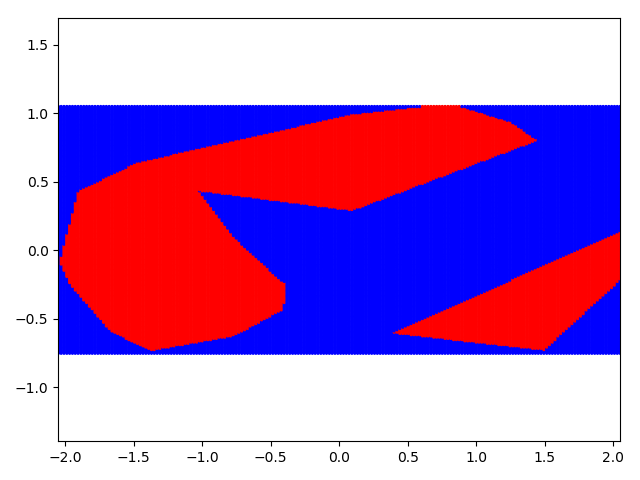
\includegraphics[scale=\myscale,scale=0.45]{figures/retro_05_p=5}
	\end{minipage}
\end{center}


\begin{center}
	\begin{minipage}{0.45\textwidth}
		\center {$p=7$, $22$ neurones, $141$ poids} 
		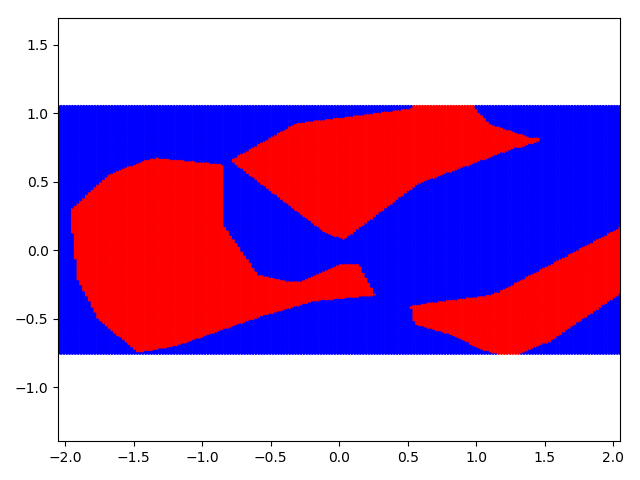
\includegraphics[scale=\myscale,scale=0.45]{figures/retro_05_p=7}
	\end{minipage}
	\begin{minipage}{0.45\textwidth}
		\center {$p=10$, $31$ neurones, $261$ poids}
		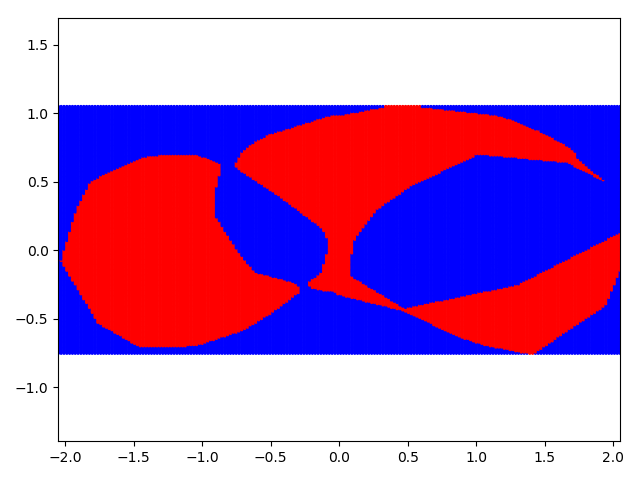
\includegraphics[scale=\myscale,scale=0.45]{figures/retro_05_p=10}
	\end{minipage}
\end{center}


\begin{center}
	\begin{minipage}{0.45\textwidth}
		\center {$p=15$, $46$ neurones, $541$ poids} 
		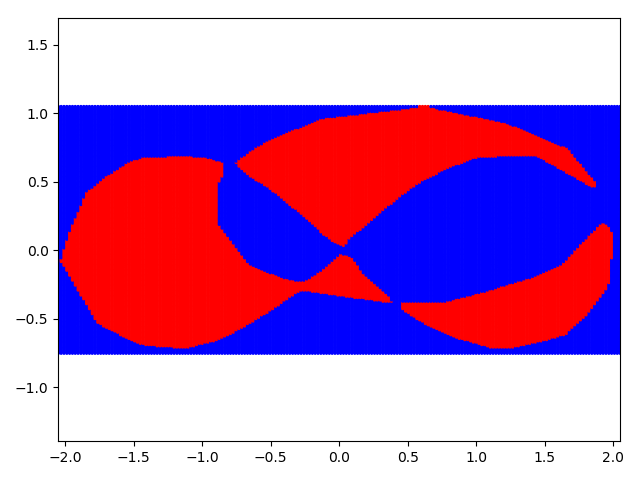
\includegraphics[scale=\myscale,scale=0.45]{figures/retro_05_p=15}
	\end{minipage}
	\begin{minipage}{0.45\textwidth}
		\center {$p=20$, $61$ neurones, $921$ poids}
		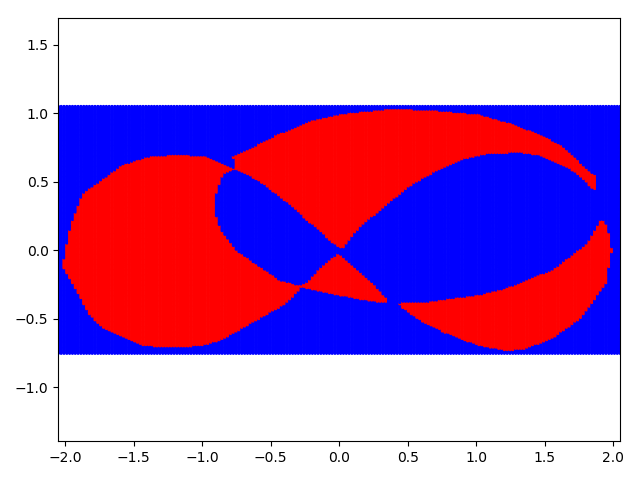
\includegraphics[scale=\myscale,scale=0.45]{figures/retro_05_p=20}
	\end{minipage}
\end{center}

\begin{center}
	\begin{minipage}{0.45\textwidth}
		\center {$p=50$, $151$ neurones, $5301$ poids} 
		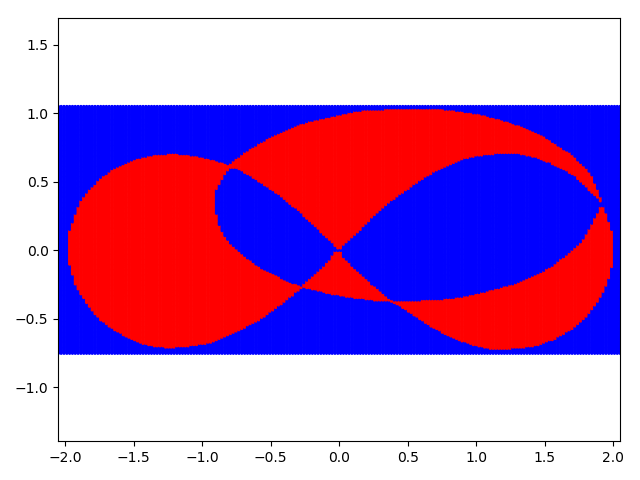
\includegraphics[scale=\myscale,scale=0.45]{figures/retro_05_p=50}
	\end{minipage}
	\begin{minipage}{0.45\textwidth}
		\center {$p=100$, $301$ neurones, $20\,601$ poids}
		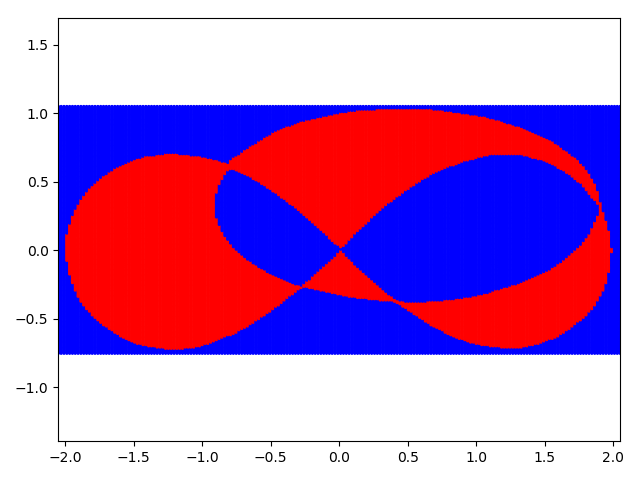
\includegraphics[scale=\myscale,scale=0.45]{figures/retro_05_p=100}
	\end{minipage}
\end{center}


Conclusion : il faut un nombre assez grand de neurones pour pouvoir modéliser des phénomènes compliqués. Dans l'exemple traité ici, on obtient une bonne approximation à partir de $p=20$, soit plus de $60$ neurones et environ $1000$ poids.


%--------------------------------------------------------------------
\subsection{Apprentissage}

N'oublions pas le but principal des réseaux de neurones : apprendre à partir des données afin de prédire des résultats pour des situations nouvelles.


Voici un problème pour lequel nous allons tester si les prédictions sur des données nouvelles sont correctes ou pas.
On dispose de $n$ cases, dont $3$ sont noircies.  On appelle \emph{hauteur}, le nombre total de cases entre la plus haute et la plus basse case noircie. Si les trois cases ont pour rang $i < j <k$ alors la hauteur vaut $h = k-i+1$ (la case noircie du milieu n'intervient pas dans la formule).
Sur le dessin ci-dessous, $n=8$ et la configuration représentée est de hauteur $6$.

\myfigure{1}{
	\tikzinput{fig_retro_12}
}

Nous voulons tester si un réseau de neurones permet de retrouver un résultat qu'on peut vérifier ici à l'aide d'une formule simple :
étant donné une configuration il s'agit de faire calculer à la machine quelle est sa hauteur. 

Il y a en tout $N = \frac{n(n-1)(n-2)}{6}$ configurations possibles pour les trois cases noires parmi $n$ cases.
On décide d'utiliser la moitié des configurations comme données d'apprentissage et l'autre moitié va nous permettre de tester si le réseau calculé avec les données d'apprentissage se comporte \og{} correctement\fg{} sur les nouvelles données.

Dans la suite nous prendrons $n=20$ cases, ce qui fait $N=1140$ configurations possibles.

\textbf{Données en entrées.}
On calcule les $N$ configurations possibles. Après un mélange aléatoire, on ne retient que $N/2$ configurations pour l'apprentissage. Une configuration est codée sous la forme d'un vecteur
$X = (x_1,x_2,\ldots,x_n)$ avec $x_i=0$ (case blanche) ou $x_i = 1$ (case noire).
Pour chaque configuration $X$ des données d'apprentissage, on calcule la hauteur $z = h(X)$. Les données d'apprentissage sont les $N/2$ données $(X_k,z_k)$ formées des entrées $X_k$ et de la sortie attendue $z_k$ correspond à la hauteur. 

\textbf{Réseau.}
Le réseau comporte $n$ entrées : une entrée par case. Il est constituée de $3$ couches.
Les deux premières couches possèdent $p$ neurones et la couche de sortie un seul. La fonction d'activation est la fonction ReLU pour tous les neurones. Sur la figure ci-dessous est illustré le cas $p=5$.

\myfigure{1}{
	\tikzinput{fig_retro_13}
}


\textbf{Apprentissage.}
Le réseau est initialisé avec des poids aléatoires. Ensuite ces poids sont modifiés par une descente de gradient stochastique avec un nombre suffisant d'itérations.

\textbf{Sortie prédite.}
Le réseau paramétré fournit une fonction $F$ à valeur réelle. La sortie attendue étant un entier, on décide que la sortie prédite sera arrondie à l'entier le plus proche.
Pour chaque $X_k$, la prédiction est correcte si la valeur arrondie $F(X_k)$ vaut la hauteur $h(X_k)$. 


\textbf{Tests.}
Il faut tester l'efficacité du réseau : tout d'abord le réseau modélise-t-il correctement les données d'apprentissage ? En effet, même si la fonction $F$ a été construite dans le but d'avoir $F(X_k) \simeq z_k$, il n'y a pas nécessairement égalité pour toutes les données d'apprentissage. Mais surtout, il faut tester si la fonction $F$ donne de bonnes prédictions pour de nouvelles données. Nous disposons pour cela des $N/2$ données de test non utilisées lors de l'apprentissage.

Les résultats dépendent des poids initiaux (aléatoires) et de la liste des configurations choisies pour l'apprentissage (liste qui a été mélangée), on ne retient que les meilleurs résultats parmi plusieurs essais.
Par exemple, pour $p=10$, voici un des meilleurs résultats obtenus :
\begin{itemize}
	\item \emph{Apprentissage.} $560$ données prédites correctement sur un total de de $570$ données d'apprentissage, soit $98\%$ de réussite.
	
	\item \emph{Test.} $506$ données prédites correctement sur un total de de $570$ données de test, soit $89\%$ de réussite.
\end{itemize}

Voici quelques résultats pour différentes valeurs de $p$.

\begin{center}
	\begin{tabular}{c|c|c|c|c}
		$p$ & {neurones} & {poids} & {pourcentage apprentissage} & {pourcentage test} \\ \hline
		3 & 7 & 79 & 50\% & 45\% \\
		5 & 11 & 141 & 85\% & 75\% \\
		7 & 15 & 211 & 90\% & 85\% \\
		10 & 21 & 331 & 98\% & 90\% \\
		15 & 36 & 571 & 99\% & 90\% \\
		20 & 41 & 861 & 100\% & 85\% \\
	\end{tabular}
\end{center}

\textbf{Commentaires.} Plus il y a de neurones, plus la fonction $F$ modélise correctement les données d'apprentissage : à partir de $20$ neurones ($p\ge10$), la modélisation est quasi-parfaite. Les pourcentages de réussite pour les données de test sont toujours inférieures et plafonnent à 90\%. Un phénomène nouveau apparaît avec plus de $40$ neurones (pour $p=20$), les pourcentages de réussite sur les tests régressent par rapport à des réseaux ayant moins de neurones, bien que les données d'apprentissage soient parfaitement modélisées : c'est un phénomène de sur-apprentissage.



%%%%%%%%%%%%%%%%%%%%%%%%%%%%%%%%%%%%%%%%%%%%%%%%%%%%%%%%%%%%%%%%%%%%%
\section{Sur-apprentissage et autres soucis}

Nous allons voir différents problèmes qui peuvent intervenir dans le calcul des poids d'un réseau de neurones, le problème le plus subtil étant le \emph{sur-apprentissage}. 


%--------------------------------------------------------------------
\subsection{Modèle insuffisant}

\textbf{Problème.}
Voici deux exemples de situations dans lesquelles le choix de l'architecture du réseau pose problème, car le réseau est trop simple. 

\bigskip

\textbf{Exemple 1.}
Imaginons que nous voulions modéliser une situation à partir des données fournies par les points $(x_i,y_i)$ du plan (figure de gauche). Si on construit un réseau d'un seul neurone (figure de droite), alors la fonction de sortie sera du type $y= F(x) = ax+b$.
\begin{center}
	\begin{minipage}{0.45\textwidth}
		\myfigure{0.7}{
			\tikzinput{fig_soucis_02}
		}
	\end{minipage}
	\begin{minipage}{0.45\textwidth}
		\myfigure{1}{
			\tikzinput{fig_soucis_01}
		}
	\end{minipage}
\end{center}

Aucun paramètre $(a,b)$ ne permettra une modélisation correcte de la situation, car les points ne sont franchement pas alignés.

\bigskip

\textbf{Exemple 2.}
Le même problème se produirait si on voulait trouver une fonction $F$, construite à partir d'un seul neurone, valant $0$ pour la zone bleue et $1$ pour la zone rouge de la figure ci-dessous. Ce n'est pas possible car la frontière de la solution n'est pas linéaire.

\begin{center}
	\begin{minipage}{0.45\textwidth}
		\myfigure{1}{
			\tikzinput{fig_soucis_03}
		}
	\end{minipage}
	\begin{minipage}{0.45\textwidth}
		\myfigure{0.7}{
			\tikzinput{fig_soucis_04}
		}
	\end{minipage}
\end{center}

\bigskip

\textbf{Conclusion.} Dans ces situations, le problème ne se situe pas au niveau des poids, augmenter la taille des données ou le nombre d'itérations n'y changera rien. La conception du réseau est mauvaise pour répondre à la question posée. C'est comme vouloir faire une course de voitures avec une deux-chevaux. La solution est de changer l'architecture du réseau, par exemple en rajoutant des neurones.

%--------------------------------------------------------------------
\subsection{Minimum local}

\index{minimum!local}

\textbf{Problème.} La descente de gradient a pour objectif de fournir un minimum local. 
Cependant rien n'affirme que ce minimum local est un minimum global.

\bigskip

\textbf{Exemple.}
Voici un réseau composé d'un seul neurone de fonction d'activation ReLU et possédant un seul coefficient à déterminer, le biais étant imposé à la valeur $-1$.
\myfigure{0.7}{
	\tikzinput{fig_soucis_08}
}
Le graphe de la fonction $F$ correspondant à ce neurone est une portion de la droite d'équation $y=ax-1$, prolongée par l'axe des abscisses. Voici l'exemple du graphe de $F$, avec $a=+2$. 

\begin{center}
	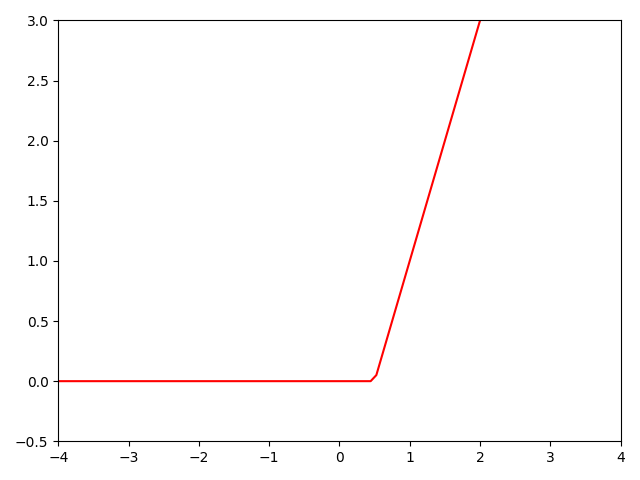
\includegraphics[scale=\myscale,scale=0.45]{figures/retro_04_d}
\end{center}

Les données sont des points déterminés par leurs coordonnées $(x_i,y_i)$ :
$$(-2,1),\quad  (-1,0),\quad (0,0),\quad (1,0),\quad (3,2).$$

\begin{center}
	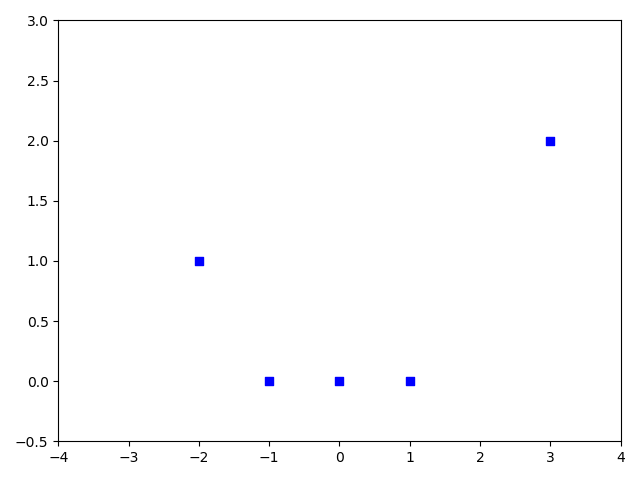
\includegraphics[scale=\myscale,scale=0.45]{figures/retro_04_a}
\end{center}

Il s'agit de trouver le meilleur coefficient $a$, qui définisse $F$ tel que $F(x_i) \simeq y_i$. Autrement dit, on souhaite minimiser $E(a) = \sum E_i(a)$ où $E_i(a) = (F(x_i)-y_i)^2$.
Géométriquement il y a deux paramètres qui semblent meilleurs que les autres $a=-1$ (figure de gauche) et $a=+1$ (figure de droite) car alors les portions de droites passent par des carrés\couleurnb{ bleus}{}.

\begin{center}
	\begin{minipage}{0.45\textwidth}
		\center \textbf{$a=-1$}
		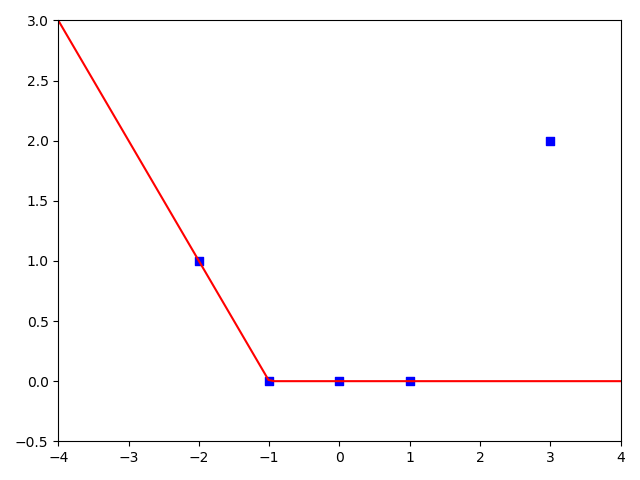
\includegraphics[scale=\myscale,scale=0.45]{figures/retro_04_b}
	\end{minipage}
	\begin{minipage}{0.45\textwidth}
		\center \textbf{$a=+1$}
		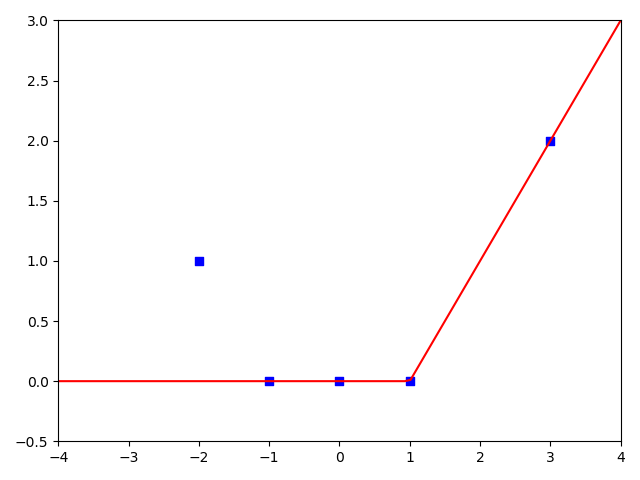
\includegraphics[scale=\myscale,scale=0.45]{figures/retro_04_c}
	\end{minipage}
\end{center}

Cette intuition se vérifie lorsque l'on trace le graphe de la fonction d'erreur $a \mapsto E(a)$. La fonction possède deux minimums locaux en $a=-1$ et $a=+1$ (et aussi une portion constante, due à l'usage de la fonction ReLU).
\begin{center}
	\textbf{Erreur $E(a)$ en fonction du coefficient $a$}
	
	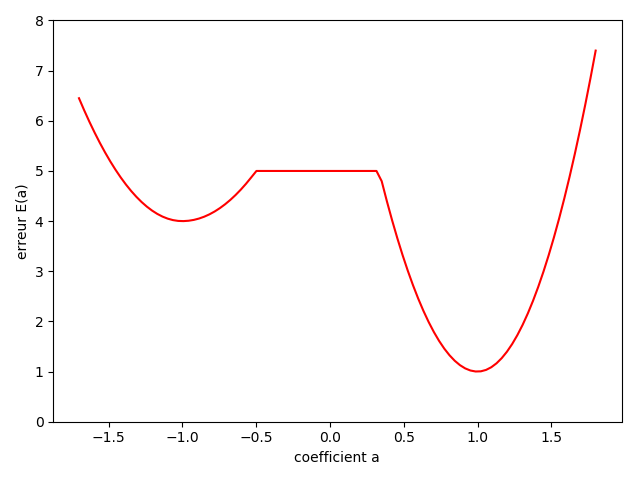
\includegraphics[scale=\myscale,scale=0.45]{figures/retro_04_e}
\end{center}
Le minimum en $a=+1$ est le minimum global. Mais si on applique la descente de gradient en partant d'un coefficient initial $a_0<0$, il y a de grandes chances d'arriver au minimum local $a=-1$, qui ne sera pas la solution optimale.

\bigskip

\textbf{Conclusion.} Vous êtes une fourmi qui se promène dans une boîte d'\oe ufs avec des trous de différentes profondeurs : vous ne pouvez pas voir à l'avance quel est l'emplacement le plus profond ! Une solution peut être de tester différentes valeurs initiales, dans le but d'obtenir différents minimums locaux.

%--------------------------------------------------------------------
\subsection{Sous-apprentissage}

\textbf{Problème.}
Le \trouer{sous-apprentissage} révèle une conception correcte de l'architecture du réseau mais une mauvaise mise en \oe uvre. On obtient alors des poids qui ne répondent pas correctement au problème.

\bigskip
\textbf{Exemple.} Une droite obtenue par un réseau approche mal une suite de points pourtant alignés.
\myfigure{0.7}{
	\tikzinput{fig_soucis_05}
}

Cela peut être dû aux raisons suivantes :
\begin{itemize}
	\item les données ne sont pas en nombre suffisant, 
	\item le nombre d'itérations est insuffisant,
	\item le pas $\delta$ est trop grand.
\end{itemize}

\bigskip

\textbf{Conclusion.} 
Il est difficile de savoir à l'avance quelle est la bonne taille
des données à utiliser et combien d'itérations sont nécessaires pour arriver à un modèle correct. Le sous-apprentissage, c'est comme faire une course de voiture avec une porsche mais en ne dépassant jamais les 80 km/h !
A posteriori, la solution est simple : ajouter des données, augmenter le nombre d'itérations ou diminuer la pas.


%--------------------------------------------------------------------
\subsection{Sur-apprentissage}

\index{sur-apprentissage}

\textbf{Problème.} Le modèle obtenu \og{}colle\fg{} parfaitement aux données d'apprentissage, mais cependant les prédictions pour de nouvelles valeurs sont mauvaises.
Il s'agit donc d'un problème délicat : la fonction $F$ obtenue vérifie bien $F(X_i) \simeq z_i$ pour toutes les données, mais pour une nouvelle entrée $X$, la sortie $F(X)$ n'est pas une bonne prédiction. Cela se produit lorsque l'on se concentre uniquement sur l'apprentissage à partir des données, mais que l'on a oublié que le but principal est la prédiction.

\bigskip

% Les exemples qui suivent ne sont pas vraiment issue de réseau de neurone, mais d'interpolation polynomiale, ce qui est plus parlant.

\textbf{Exemple 1.} Nous avons $4$ points\couleurnb{ bleus}{}.
Pour une valeur $x_0$ donnée, on souhaite prédire une valeur $y_0$ (figure de gauche) cohérente avec nos données.

On propose dans un premier temps d'approcher la solution en utilisant une droite (figure de droite) même si les points ne sont pas exactement alignés. Cela permet de prédire une valeur $y_0$ pour placer le point $P=(x_0,y_0)$.
Ce modèle ne sera jamais parfait car les points ne sont pas alignés, donc aucune droite ne convient exactement, autrement dit l'erreur ne sera jamais nulle.

\myfigure{0.7}{
	\tikzinput{fig_soucis_06a}
	\tikzinput{fig_soucis_06b}
}

On peut construire un modèle plus compliqué, par exemple chercher une courbe polynomiale de degré $3$ ou plus qui passe \emph{exactement} par tous les points d'apprentissage. Ainsi, pour cette courbe, l'erreur sera nulle. Cette courbe permet de prédire une valeur $y_0'$ pour placer un point $P'(x_0,y_0')$. 

\myfigure{0.8}{
	\tikzinput{fig_soucis_06c}
}
Ce dernier modèle répond entièrement au problème, mais la solution proposée ne semble pas raisonnable par rapport aux données de départ. C'est un cas de sur-apprentissage : le modèle est correct sur les données, mais les prédictions seront mauvaises.

\bigskip

\textbf{Exemple 2.}
Le problème est similaire si on essaye de séparer les ronds bleus des carrés rouges de la figure de gauche ci-dessous. Une modèle simple permet à une parabole de séparer l'essentiel des ronds bleus des carrés rouges (figure centrale). On peut entraîner un modèle plus complexe pour qu'il délimite parfaitement les deux types de points, mais au prix d'une complexité non nécessairement voulue (figure de droite).
\myfigure{0.7}{
	\tikzinput{fig_soucis_07a}\qquad
	\tikzinput{fig_soucis_07b}\qquad
	\tikzinput{fig_soucis_07c}
}

\textbf{Conclusion.}
Le sur-apprentissage, c'est comme emmener ses enfants à l'école en conduisant à 200 km/h : cela répond de façon correcte à un problème, mais cela provoque beaucoup d'autres ennuis !  
Quelle est la meilleure solution entre un modèle simple mais imparfait et un modèle parfait mais compliqué ? Il n'y a pas une réponse immédiate à la question : pour le savoir, il faut tester le modèle sur d'autres données, jamais rencontrées précédemment, afin de déterminer si le réseau n'a pas été sur-entraîné.
